% COGNITIVE GRAPH THEORY - REVISED VERSION
% Author: Zeng Mingjia
% Date: \today

\documentclass[12pt,a4paper]{article}
\usepackage[UTF8]{ctex}
\usepackage{amsmath,amssymb,amsthm}
\usepackage{graphicx}
\usepackage{booktabs}
\usepackage{multirow}
\usepackage{algorithm}  % 算法环境
\usepackage{algpseudocode}  % 替换 algorithmicx，提供更好的伪代码支持
\usepackage{enumitem}
\usepackage{listings}
\usepackage{xcolor}
\usepackage{caption}
\usepackage{subcaption}
\usepackage{longtable}
\usepackage{arydshln}
\usepackage{float}
\usepackage[sort&compress]{natbib}  % 更强大的引用管理，替换原来的 cite 包
\bibliographystyle{plainnat}  % 引用样式，也可以选 apalike, ieeetr, alpha 等
\usepackage{tikz}
\usetikzlibrary{backgrounds,trees,positioning, shapes,shapes.misc,shadows,  arrows.meta,arrows, calc, decorations.pathreplacing,mindmap}
\usepackage{pgfplots}  % 如果使用坐标轴
\pgfplotsset{compat=1.17}
\usepackage{array}  % 增强表格功能
\usepackage{booktabs}  % 三线表
\usepackage{makecell}  % 多行表头
\usepackage{multirow}  % 多行合并
\usepackage[top=2.5cm, bottom=2.5cm, left=2.5cm, right=2.5cm]{geometry}
% 定义常用列类型
\newcolumntype{C}{>{\centering\arraybackslash}p}  % 居中的固定宽度列
\newcolumntype{L}{>{\raggedright\arraybackslash}p}  % 左对齐的固定宽度列
\newcolumntype{R}{>{\raggedleft\arraybackslash}p}  % 右对齐的固定宽度列

% 小型表格样式
\newcommand{\smalltable}{\scriptsize}
% 算法命令定义 - 修正
\renewcommand{\algorithmicrequire}{\textbf{输入:}}
\renewcommand{\algorithmicensure}{\textbf{输出:}}
\renewcommand{\algorithmiccomment}[1]{\{#1\}}



% 代码样式设置
\lstset{
    basicstyle=\ttfamily\small,
    keywordstyle=\color{blue},
    commentstyle=\color{green},
    stringstyle=\color{red},
    numbers=left,
    numberstyle=\tiny\color{gray},
    stepnumber=1,
    numbersep=5pt,
    backgroundcolor=\color{white},
    showspaces=false,
    showstringspaces=false,
    showtabs=false,
    frame=single,
    rulecolor=\color{black},
    tabsize=2,
    captionpos=b,
    breaklines=true,
    breakatwhitespace=false,
    escapeinside={\%*}{*},
}

% 数学命令
\newcommand{\cognitivespace}{\mathcal{C}}
\newcommand{\cognitivegroup}{\mathbb{G}}
\newcommand{\energyoperator}{\mathcal{E}}
\newcommand{\compressionoperator}{\mathcal{C}}
\newcommand{\migrationoperator}{\mathcal{M}}

% hyperref 最后加载
\usepackage{hyperref}

% 标题
\title{认知的几何、代数与动力学：基于能耗最小化原理的统一图论模型}
\author{曾铭佳}
\date{\today}

\begin{document}

\maketitle

\begin{abstract}
回应Bowers等人（2023）对认知模型方法论的要求，本文构建一个基于第一性原理的思想实验平台，从几何、代数和动力学三个维度为认知过程提供统一的形式化描述。系统建立在两个核心公设之上：(1) 认知状态可表征为时空中的动态网络（认知图）；(2) 网络演化受能量动力学支配，其核心优化目标是认知自由能（广义认知能耗）最小化。在此框架下，我们引入群论结构以描述认知操作的封闭性和可逆性，并观察到“概念压缩”与“第一性原理迁移”可作为系统能耗优化的自然产物而涌现。

为观察公理系统的内生行为，我们在包含51至111个跨领域概念的网络上进行思想实验。结果显示，由核心公设驱动的“自然涌现模型”在不同规模下均可实现显著的能耗降低（47.9\%-86.9\%），优于外部干预的预设模型。进一步地，我们观察到系统演化遵循一系列可量化的宏观规律：能耗随迭代呈幂律衰减（$R^2\approx1.0$）；被压缩概念集群的内部-外部能耗比（压缩势）稳定在0.8左右；概念在压缩事件中的出现频率服从幂律分布（斜率约-1.35），这与复杂系统的无标度特征和人类语言使用的Zipf定律相呼应。这些观察为能量最小化作为认知组织基本原则提供了多维度的计算证据，并展示了从少数原理出发描述知识内化与创造性思维涌现的可行性。本工作旨在为理解智能的本质提供一个基于原理的数学视角，而非构建可直接应用的工程系统。

\textbf{关键词：} 认知图论，能量最小化，思想实验，概念压缩，幂律分布，认知动力学
\end{abstract}

\newpage
% ========== SECTION 1: 引言 ==========
\section{引言}

构建一个能够同时描述知识表征、学习动态与创造性思维的计算理论，是认知科学与人工智能领域的核心挑战。现有工作，如语义网络与知识图谱，精于描述知识的静态结构，却拙于刻画其动态演化过程与内在的优化目标。当前人工智能系统，特别是大型语言模型，虽然在特定任务上表现出色，但其运作机制本质上仍是基于统计关联的暴力计算，这限制了其在创造性思维、跨领域迁移和能量效率方面的表现。

本文采取一条与主流研究截然不同的路径。我们的目标并非构建一个能与人类行为数据精确拟合的工程模型，也无意与现有AI系统进行性能对标。相反，我们希望建立一个基于第一性原理的思想实验平台。在这个由少数简洁公设（认知时空与能量动力学）定义的计算宇宙中，我们可以观察并描述认知组织的基本原则如何从微观互动中自发产生。近期，Bowers等人 \cite{bowers2023importance} 对深度学习模型与人类认知的对比研究提出了深刻的方法论批评。本文从一个不同角度回应这一问题：不是通过改进实证检验的方法，而是通过从第一性原理出发构建一个可计算的思想实验平台，探索认知组织的基本原则。在这个意义上，本文是对Bowers等人呼吁的一种正面建设性回应。

受物理学中最小作用量原理的启发，本文提出一个核心论点：认知过程的底层驱动力，是对“认知能耗”这一内部代价的优化。基于此，我们构建了一个以“认知时空”与“能量动力学”为第一性原理的公理化系统。为给这个动态系统提供更严格的数学基础，我们进一步引入了群论结构，探讨认知操作在复合下构成半群的可能性，并观察认知对称性与守恒量之间可能存在的对应关系。

本文的主要理论探索包括：
\begin{itemize}
\item 建立认知图论的完整公理化体系，包含几何、代数和动力学三个维度。
\item 引入群论结构描述认知操作的代数性质，并通过计算实验探讨其可行性。
\item 提出并对比两种研究范式：代表外部干预的“预设算法设计”与代表自组织的“自然能量涌现”。
\item 通过能耗下降曲线拟合、概念出现频率的幂律检验、压缩势分析等多维度客观指标，观察“概念压缩”和“第一性原理迁移”等现象的涌现规律，为理论的认知合理性提供可量化的观察窗口。
\end{itemize}

\textbf{研究范式定位：} 需要特别说明的是，本研究并非旨在构建一个能够精确拟合人类行为数据的认知模型。Woensdregt等人 \cite{woensdregt2024lessons} 曾指出，在实证证据稀疏或间接的领域，理论发展需要遵循“良性实践”。本文的工作可以看作是在认知计算建模领域对这些实践的一次具体应用：我们明确陈述两个公设，梳理并对比现有理论，构建可计算模型进行思想实验，并寻求模型行为与多个认知理论及统计规律的外部一致性。这一方法论立场贯穿全文。

% ========== SECTION 2: 相关工作和理论背景 ==========
\section{相关工作和理论背景}

% ========== SUBSECTION 2.1: 认知计算模型的主要流派与理论脉络 ==========
\subsection{认知计算模型的主要流派与理论脉络}

认知计算模型的发展经历了从符号主义到连接主义的范式演进，同时涌现出能量优化视角、代数/几何方法以及复杂系统视角等多种理论探索。

\textbf{符号主义模型}（如ACT-R \cite{anderson2004act}、SOAR）擅长基于规则的符号处理，但在面对复杂、模糊的真实世界情境时，往往面临组合爆炸问题，其产生式系统难以模拟人类思维的流畅性与灵活性。

\textbf{连接主义模型}，特别是以Transformer架构\cite{vaswani2017attention}和大型语言模型为代表的深度学习\cite{lecun2015deep}，通过神经网络的分布式表征取得了突破性进展。这些模型在感知和模式识别任务上表现优异，但本质上仍是对统计关联的拟合，其运作机制常被视为“黑箱”，难以解释驱动认知结构演化的内在原理。

\textbf{能量优化视角}受到Karl Friston自由能原理\cite{friston2010free}的启发，认为大脑通过最小化预测误差来维持内稳态。Tenenbaum的概念生长理论\cite{tenenbaum2011grow}和Gärdenfors的概念空间理论\cite{gardenfors2004conceptual}分别从贝叶斯和几何角度刻画概念学习，但主要关注静态结构或概率推理，对驱动认知结构演化的能量动力学机制探讨较少。近期Tankut Can \cite{can2025statistical}从统计力学研究语义压缩，与本文的能量最小化框架形成平行对话。

\textbf{代数与几何方法}方面，群论\cite{rotman1995theory}在认知科学中已有初步探索，如Shepard的心理旋转实验，但多停留在现象描述。Gärdenfors的概念空间理论提供了几何描述，但缺乏对认知操作代数结构的系统整合。Glazebrook与Wallace \cite{glazebrook2009small}曾用群胚描述认知网络中的对称性与轨道等价关系，其驱动力来自信息论，与本文的能耗最小化公设不同。

\textbf{复杂系统视角}强调宏观秩序模式可从微观元素的简单相互作用中自发产生，为理解创造性思维等高阶认知功能提供了新思路，但现有研究多停留在定性描述，缺乏基于第一性原理的可计算涌现模型。

% ========== SUBSECTION 2.2: 研究启发与本工作的理论定位 ==========
\subsection{研究启发与本工作的理论定位}
\label{subsec:research_gaps_positioning}

综合上述脉络，可以看到现有理论在整合性、原理性、机制性、涌现性等方面仍有待深入探索。本工作尝试围绕这些问题展开探索，从以下角度构建一个以能量最小化为第一性原理的认知计算框架：
\begin{enumerate}
\item \textbf{整合几何、代数与动力学}：通过动态网络描述几何结构，引入群论刻画代数性质，基于能量动力学驱动演化。
\item \textbf{从公设推导认知现象}：从“认知时空”与“能量动力学”两个核心公设出发，探讨“概念压缩”和“第一性原理迁移”作为能耗优化结果的自然涌现。
\item \textbf{机制探索与涌现观察}：通过计算实验观察能量优化如何塑造认知结构，并对比预设算法模型与自然涌现模型，观察复杂行为从简单规则中产生的过程。
\end{enumerate}

\textbf{理论定位}：与现有研究相比，本文工作的独特之处在于：(1) 核心论点：认知的底层驱动力是对“认知能耗”这一内部代价的优化；(2) 公理化路径：从简单公设出发构建数学框架并观察其衍生现象；(3) 可计算的思想实验：通过计算实验在可控环境中观察理论预测的行为模式。

因此，本工作并非要取代现有理论，而是提供一个可供观察和思考的“认知宇宙”，为理解知识内化到灵感涌现的认知谱系提供新的视角。

% ========== SUBSECTION 2.3: 理论背景示意图 ==========
\subsection{与现有认知理论的对比}
\label{subsec:comparison_with_existing}

为更清晰地定位本工作的理论贡献，本节简要对比认知图论与主要现有认知理论的关系。

\begin{itemize}
\item \textbf{与符号主义模型的对比}：符号主义模型擅长基于规则的符号处理，但面临组合爆炸问题。认知图论通过能量优化的网络演化，为符号操作提供了连续、可学习的底层动力学，二者可在逻辑推理与灵活思维之间形成互补。
\item \textbf{与连接主义模型的对比}：深度神经网络在感知和模式识别上表现优异，但其统计关联的本质使其难以解释认知结构的内在原理。认知图论的代数结构为网络黑箱提供了可解释的数学语言，而能量最小化则为学习提供了内在驱动。
\item \textbf{与自由能原理的对比}：本工作与Friston的自由能原理共享“能量最小化”核心原则，但研究层次与实现机制不同。自由能原理旨在解释神经层面的预测处理，是一个深刻的哲学框架；认知图论则在认知抽象层面构建了具体的、可操作的动力学系统。两者可视为不同层次上的平行探索。
\item \textbf{与概念空间理论的对比}：Gärdenfors的概念空间理论为概念表征提供了优雅的几何框架，但缺乏动态演化和代数描述。认知图论在此基础上增加了能量驱动的网络演化和群论代数结构。
\item \textbf{与Glazebrook \& Wallace认知几何模型的对比}：Glazebrook与Wallace使用群胚描述认知网络中的局部对称性，其动力学由信息论驱动。本文从能耗最小化公设出发，使用群论描述认知操作的代数结构，关注概念压缩与原理迁移的涌现，体现了代数几何语言在认知建模中的广泛适用性。
\end{itemize}

% ========== SUBSECTION 2.4: 理论背景示意图 ==========
\subsection{理论背景示意图}
\label{subsec:theoretical_background_mindmap}

为直观展示本章所讨论的理论脉络，图\ref{fig:theoretical_background_mindmap}以思维导图形式汇总了相关工作的演进路径、核心概念与本文的理论定位：

\begin{figure}[H]
\centering
\begin{tikzpicture}[
    scale=0.75,
    mindmap,
    every node/.style={concept, execute at begin node=\hskip0pt, align=center, draw, rectangle, rounded corners=3pt, font=\small},
    level 1 concept/.append style={level distance=4.5cm, sibling angle=120, font=\normalsize\bfseries},
    level 2 concept/.append style={level distance=3.5cm, sibling angle=45, font=\small},
    level 3 concept/.append style={level distance=2.5cm, sibling angle=30, font=\footnotesize},
    text=black
]

% 中心主题：认知计算理论
\node[concept, fill=blue!20, text width=2.5cm] {认知计算理论\\脉络与探索}
    [clockwise from=0]
    child[concept color=green!30, grow=30] {
        node[concept, fill=green!20, text width=2.5cm] {符号主义模型\\[2pt]ACT-R, SOAR}
        child[grow=60] {
            node[concept, fill=green!10, text width=2.0cm] {基于规则\\符号处理}
        }
        child[grow=30] {
            node[concept, fill=green!10, text width=2.0cm] {产生式系统\\逻辑推理}
        }
        child[grow=0] {
            node[concept, fill=green!10, text width=2.0cm] {组合爆炸\\灵活性局限}
        }
    }
    child[concept color=orange!30, grow=90] {
        node[concept, fill=orange!20, text width=3cm] {连接主义模型\\[2pt]深度学习, Transformer}
        child[grow=120] {
            node[concept, fill=orange!10, text width=2.0cm] {统计关联\\分布表征}
        }
        child[grow=90] {
            node[concept, fill=orange!10, text width=2.0cm] {大规模预训练\\模式识别}
        }
        child[grow=60] {
            node[concept, fill=orange!10, text width=2.0cm] {可解释性挑战\\缺乏原理}
        }
    }
    child[concept color=purple!30, grow=150] {
        node[concept, fill=purple!20, text width=3cm] {能量优化视角\\[2pt]自由能原理}
        child[grow=180] {
            node[concept, fill=purple!10, text width=2.0cm] {预测误差最小化\\主动推理}
        }
        child[grow=150] {
            node[concept, fill=purple!10, text width=2.0cm] {神经层面原理\\变分贝叶斯}
        }
        child[grow=120] {
            node[concept, fill=purple!10, text width=2.0cm] {认知层面机制\\尚待具体化}
        }
    };

% 第二圈分支
\node[concept, fill=yellow!20, text width=3.0cm] at (330:5) {代数/几何方法\\[2pt]概念空间, 群论}
    [clockwise from=270]
    child[concept color=yellow!30, grow=300] {
        node[concept, fill=yellow!10, text width=2.0cm] {概念空间理论\\几何表征}
    }
    child[concept color=yellow!30, grow=330] {
        node[concept, fill=yellow!10, text width=2.0cm] {群论结构\\认知对称性}
    }
    child[concept color=yellow!30, grow=360] {
        node[concept, fill=yellow!10, text width=2.0cm] {动态演化\\有待整合}
    };

% 第三圈分支
\node[concept, fill=red!20, text width=3.0cm] at (210:5) {复杂系统视角\\[2pt]涌现现象}
    [clockwise from=210]
    child[concept color=red!30, grow=180] {
        node[concept, fill=red!10, text width=2.0cm] {自组织\\临界现象}
    }
    child[concept color=red!30, grow=210] {
        node[concept, fill=red!10, text width=2.0cm] {从简单规则\\产生复杂行为}
    }
    child[concept color=red!30, grow=240] {
        node[concept, fill=red!10, text width=2.0cm] {可计算模型\\有待发展}
    };

% 理论定位（下方中心）
\node[concept, fill=gray!20, text width=4cm] at (0,-5) {\textbf{本文理论定位：思想实验平台}}
    child[concept color=gray!30, grow=-90] {
        node[concept, fill=gray!10, text width=3.0cm, align=center] {
            \textbf{整合几何、代数、动力学}\\
            统一的形式框架
        }
    }
    child[concept color=gray!30, grow=-30] {
        node[concept, fill=gray!10, text width=3.0cm, align=center] {
            \textbf{基于第一性原理}\\
            从公设推演现象
        }
    }
    child[concept color=gray!30, grow=-150] {
        node[concept, fill=gray!10, text width=3.0cm, align=center] {
            \textbf{可计算的涌现观察}\\
            思想实验验证
        }
    };

\end{tikzpicture}
\caption{相关理论背景脉络图：展示了符号主义、连接主义、能量优化、代数/几何方法和复杂系统等主要理论方向的核心观点与待探索之处，以及本文的思想实验定位。}
\label{fig:theoretical_background_mindmap}
\end{figure}

图\ref{fig:theoretical_background_mindmap}以可视化形式呈现了本章的核心内容，突出了现有理论的贡献与开放问题，并点明本文作为思想实验平台的独特定位。

% ========== SECTION 3: 认知图论的公理系统：几何描述 ==========
\section{认知图论的公理系统：几何描述}

本节为认知图论搭建几何层面的公理基础。我们将认知状态视作动态网络，并引入能量动力学作为其演化的第一性原理。从这两个基本公设出发，可以观察到系统呈现出一系列衍生性质，如可迭代性和可回归性。这些性质并非人为设定，而是公设的必然结果，它们为理解认知过程的连续性与稳定性提供了几何视角。

% ========== SUBSECTION 3.1: 基本公设 ==========
\subsection{基本公设}

\textbf{公设一：认知时空（几何表述）}

存在一个认知网络 $G(V,E,t)$，其中：
\begin{itemize}
\item $V = \{v_1, v_2, \ldots, v_n\}$ 是概念节点集合，每个节点 $v_i$ 代表一个基本概念或知识单元。
\item $E \subseteq V \times V$ 是概念关联边集合，每条边 $e_{ij} = (v_i, v_j)$ 代表概念间的语义或功能关联。
\item $t \in \mathbb{R}^+$ 是连续时间参数，网络的拓扑结构 $\Gamma(t)$ 和连接权重 $w_{ij}(t)$ 都随时间演化。
\end{itemize}

这个动态网络构成了认知活动发生的“舞台”，每个认知状态对应网络的一个特定几何配置。网络的几何特性包括度分布 $P(k)$、聚类系数 $C$、路径长度 $L$、模块性 $Q$ 等。

\textbf{公设二：能量动力学（几何表述）}

认知网络的演化受能量动力学支配：

\begin{enumerate}
\item \textbf{认知能耗函数}：对于任意边 $e_{ij} \in E$，存在认知能耗函数：
\begin{equation}
E_{ij}(t) = f(\Delta_{ij}, s_{ij}, h_{ij}(t), \Theta)
\end{equation}
其中 $\Delta_{ij}$ 是节点间的结构差异性，$s_{ij}$ 是语义关联强度，$h_{ij}(t)$ 是遍历历史熟练度，$\Theta$ 是个体认知参数。

\item \textbf{能耗演化机制}：边的能耗动态受历史遍历调控：
\begin{equation}
E_{ij}(t+1) = g(E_{ij}(t), H_{ij}(t), \Theta)
\end{equation}
其中 $H_{ij}(t)$ 是历史遍历记录。

\item \textbf{优化方向}：系统长期演化趋向于最小化全局认知自由能：
\begin{equation}
F(G) = \sum_{e_{ij} \in E} E_{ij} - T \cdot S(G) + R(G)
\end{equation}
其中 $S(G)$ 是网络的结构熵，$T$ 是认知温度参数，$R(G)$ 是认知资源约束函数。
\begin{small}
    后文中为行文简洁，常以“认知能耗”泛指这一广义自由能，但数学上的优化目标始终为$F(G)$。
\end{small}


\end{enumerate}

\begin{figure}[H]
\centering
\begin{tikzpicture}[
    scale=1.0,
    every node/.style={circle, draw, minimum size=1.2cm},
    concept/.style={fill=blue!20},
    energy/.style={fill=red!20},
    thick,
    >=stealth
]

% 定义节点位置
\node[concept] (v1) at (-2,1) {算法};
\node[concept] (v2) at (1,2) {递归};
\node[concept] (v3) at (3,1) {神经网络};
\node[concept] (v4) at (0,-2) {模式识别};
\node[concept] (v5) at (4,-2) {优化};
\node[energy] (v6) at (7,-3) {认知能耗};

% 连接边并标注权重
\draw[->] (v1) -- node[midway, above left] {0.85} (v2);
\draw[->] (v1) -- node[midway, above] {0.78} (v3);
\draw[->] (v2) -- node[midway, right] {0.92} (v3);
\draw[->] (v2) -- node[midway, left] {0.67} (v4);
\draw[->] (v3) -- node[midway, right] {0.81} (v5);
\draw[->] (v4) -- node[midway, below] {0.74} (v5);
\draw[->] (v5) -- node[midway, right] {0.63} (v6);
\draw[->] (v1) .. controls (-1,1) and (-1,-1) .. node[midway, left] {0.45} (v4);
\draw[->] (v3) .. controls (5,1) and (5,-1) .. node[midway, right] {0.58} (v5);

% 标注
\node[text width=4cm, align=center, font=\small] at (6,4) {认知图 $G(V,E,t)$ \\ 时间 $t$: 迭代次数};
\node[text width=3cm, align=center, font=\small] at (-1,4) {节点: 概念 \\ 边权重: 认知能耗};

% 能量函数示意
\node[rectangle, draw, rounded corners, fill=yellow!20, minimum width=6cm, minimum height=1.5cm, text width=5.5cm, align=left] at (7,1) {
    \textbf{认知能耗函数:} \\
    $E_{ij}(t) = \alpha(1-\text{sim}_{ij}) + \beta\frac{1}{1+H_{ij}(t)} + \gamma\cdot\text{div}_{ij}$ \\
    $\alpha=0.4,\ \beta=0.4,\ \gamma=0.2$
};

\end{tikzpicture}
\caption{认知图的基本结构：节点表示概念，边表示概念间的关联，边权重表示认知能耗。图中展示了算法、递归、神经网络等概念及其关联，认知能耗函数将能耗分解为语义差异、历史熟练度和结构差异三部分。}
\label{fig:cognitive_graph_structure}
\end{figure}

注：认知图论选择图论作为基础框架，是因为图论能够自然表达概念的语境依赖性——同一节点在不同子图中可扮演不同角色（整体或部分），并且可以通过边的动态变化模拟认知演化。

% ========== SUBSECTION 3.2: 几何衍生性质 ==========
\subsection{几何衍生性质}

下述性质并非独立假设，而是上述公设的必然推论，反映了系统在公设下自然呈现的行为模式。

\textbf{性质1：可迭代性（几何表述）}

认知时空 $G(V,E,t)$ 的动态性由其自身的演化方程定义：
\begin{equation}
G(t+1) = \Phi(G(t), I(t), \Theta)
\end{equation}
其中 $\Phi$ 是认知演化算子，$I(t)$ 是外部输入，$\Theta$ 是系统参数。这一迭代过程将历史状态与新输入整合，依据能量动力学优化网络几何结构。

\textbf{性质2：可回归性（几何表述）}

系统的任何状态 $G(t)$ 都是其构建历史的完整几何记录，可形式化为：
\begin{equation}
G(t) = F(A_1, A_2, \ldots, A_t; G(0))
\end{equation}
其中 $A_i$ 是历史算法操作序列，$G(0)$ 是初始状态。这意味着当前几何状态是其全部历史的“路径积分”，可回归性正是这一路径依赖特性的外在表现，解释了复习为何能快速恢复熟练度。

分析上述两种性质可知，可迭代性与可回归性均由时间维度引入，即动力学带来的结果。原本静态的图因时间维度而演化，每个节点概念在时间轴上的演化轨迹构成了认知的可回归基础。

% ========== SUBSECTION 3.3: 数学形式化 ==========
\subsection{数学形式化}
为使理论更具可计算性与可验证性，本节给出核心概念的数学形式化描述，为后续思想实验中观察和测量认知现象提供基础。

\textbf{认知能耗函数}：为将公设二具体化，定义边 $e_{ij}$ 在时刻 $t$ 的认知能耗函数为：
\begin{equation}
E_{ij}(t) = \alpha \cdot (1 - \text{sim}(v_i, v_j)) + \beta \cdot \frac{1}{1 + H_{ij}(t)} + \gamma \cdot \text{div}(v_i, v_j)
\label{eq:energy_function}
\end{equation}
其中 $\text{sim}(v_i, v_j) \in [0, 1]$ 表示节点间的语义或结构相似度，$H_{ij}(t)$ 是到时刻 $t$ 为止边的遍历次数（历史熟练度），$\text{div}(v_i, v_j)$ 是结构差异性，$\alpha, \beta, \gamma$ 为权重参数且 $\alpha + \beta + \gamma = 1$。

\textbf{概念压缩的触发条件}：节点集合 $C = \{v_1, \ldots, v_k\}$ 可被压缩为一个宏观节点 $v_C$，当且仅当满足：
\begin{equation}
\frac{1}{|C|}\sum_{v_i \in C} \overline{E_{i, \text{external}}} > \theta_c \cdot (E_{C, \text{internal}} + \overline{E_{C, \text{external}}})
\label{eq:compression_condition}
\end{equation}
其中 $\overline{E_{i, \text{external}}}$ 是 $C$ 内节点与外部连接的平均能耗，$E_{C, \text{internal}}$ 是压缩后维持内部结构的能耗，$\overline{E_{C, \text{external}}}$ 是压缩后与外部连接的平均能耗，$\theta_c > 1$ 是压缩触发阈值。此不等式表明，当维持分散结构的平均外部能耗高于压缩后总能耗的阈值时，压缩成为能量最优解。

% ========== SUBSECTION 3.4: 集群压缩势：一种连续度量指标 ==========
\subsection{集群压缩势：一种连续度量指标}
\label{subsec:compression_potential}

为更精细地刻画概念压缩现象的内在能量特征，我们引入一个连续指标——集群压缩势（Compression Potential）。对于任意候选节点集合 $C \subseteq V$，定义其压缩势为：
\begin{equation}
\Phi(C) = \frac{\overline{E}_{\text{internal}}(C)}{\overline{E}_{\text{external}}(C)}
\label{eq:compression_potential}
\end{equation}
其中 $\overline{E}_{\text{internal}}(C)$ 是集合 $C$ 内部所有连边的平均认知能耗，$\overline{E}_{\text{external}}(C)$ 是 $C$ 中节点与外部节点（$V \setminus C$）之间所有连边的平均认知能耗。$\Phi(C)$ 的值越小，表明该集群内部连接越紧密（能耗低）、外部连接越松散（能耗高），因此压缩该集群所能获得的能耗收益预期越大。

压缩势是一个纯粹的观测指标，它不参与系统的演化决策，仅用于事后分析被系统实际压缩的集群的统计特征。它与第 3.3 节中定义的压缩触发条件（公式 \ref{eq:energy_function} 及后续说明）本质上是等价的——压缩势反映了集群内部与外部的能耗对比，而触发条件则是该对比超过某一阈值时的具体表现。引入压缩势使我们能够以连续、客观的方式考察压缩行为的质量，并为第 7.3 节的规模效应分析提供量化依据。

% ========== SUBSECTION 3.5: 认知遍历的几何理论 ==========
\subsection{认知遍历的几何理论}

作为能量动力学的操作实现，系统演化依赖于两种基本的认知遍历模式，它们对应在认知空间中的不同运动方式。

\textbf{定义3.5.1（硬遍历）}：系统沿已有低能耗路径进行精确、高效的思维操作，路径确定性高、能耗较低，服务于知识的巩固和应用。几何上表现为在已知低维流形上的运动。

\textbf{定义3.5.2（软遍历）}：系统以较高探索性代价搜索新或弱关联路径，路径随机性强、能耗较高，服务于知识的探索和创新。几何上表现为在高维或未知区域的探索。

% ========== SUBSECTION 3.6: 全文语境假设 ==========
\subsection{全文语境假设}

本研究的理论框架与实验设计基于一个明确的前提假设：所有认知活动发生在\textbf{单一静态语境}之中。所谓单一静态语境，是指在同一认知场景下，概念节点及其关联边所构成的网络结构不因语境切换而改变，整个演化过程均在一个固定的“认知舞台”上展开。这类似于物理学中研究理想气体时所采用的“孤立系统”假设——虽然现实气体总会与外界交换能量，但孤立系统的简化使我们能首先揭示压强、温度等核心变量的基本规律。

现实中的认知过程总是高度语境依赖的，但若在建模之初即引入多语境机制，将同时面临概念表征的动态演化与语境切换的双重复杂性，难以清晰剥离能量最小化原则本身的作用。因此，我们首先在单一静态语境下建立基础模型，专注于观察“认知能耗最小化”这一核心驱动力如何塑造认知结构，待基本规律明晰后再逐步融入语境维度。

尽管当前采用静态语境假设，但图论本身为动态语境的建模预留了接口：可引入语境节点、动态边权重受语境调制、语境演化算子等。因此，本工作所建立的静态语境模型是迈向动态语境认知模拟的第一步。

% ========== SECTION 4: 认知图论的代数结构：群论描述 ==========
\section{认知图论的代数结构：群论描述}

在前一节中，我们从几何层面将认知状态刻画为动态网络。本节尝试引入代数工具，为认知操作提供更结构化的描述。群论作为研究对称性和变换的数学语言，可以帮助我们理解认知操作之间的组合关系、可逆性以及可能存在的守恒量。需要说明的是，这里提出的代数结构是一种形式化尝试，旨在为后续的认知动力学分析提供一个抽象的数学视角，而不是在断言现实认知必然严格遵循群的所有公理。

\subsection{认知操作的代数系统}

为给认知图论提供更丰富的数学描述，我们考虑用代数结构来刻画基本认知操作之间的相互关系。

设 $\cognitivespace$ 为所有可能认知状态的集合，即 $\cognitivespace = \{G(V,E,t) | t \in \mathbb{R}^+\}$。基本认知操作包括遍历 $\tau$、学习 $\lambda$、遗忘 $\phi$、压缩 $\kappa$、迁移 $\mu$ 等。这些操作的集合在复合运算下构成一个半群：任意两个操作的复合仍是一个认知操作，且复合满足结合律（但不一定满足交换律）。单位元对应“空操作”（保持状态不变）。这一结构为理解认知过程的组合性质提供了代数基础。

\begin{figure}[H]
\centering
\begin{tikzpicture}[
    scale=0.70,
    operation/.style={rectangle, draw, rounded corners, minimum width=2.2cm, minimum height=1cm, align=center},
    op1/.style={fill=blue!20},
    op2/.style={fill=green!20},
    op3/.style={fill=orange!20},
    result/.style={fill=red!20},
    space/.style={rectangle, draw, rounded corners, fill=gray!10, minimum width=4cm, minimum height=2cm},
    thick,
    >=stealth,
    node distance=1.5cm
]

% 操作节点
\node[operation, op1] (tau) at (0,3) {遍历 $\tau$};
\node[operation, op2, right=of tau] (lambda) {学习 $\lambda$};
\node[operation, op3, right=of lambda] (phi) {遗忘 $\phi$};

% 复合操作
\node[operation, result, below=2cm of lambda] (composite) at (3,0.5) {复合操作 $\phi\circ\lambda\circ\tau$};

% 连接线表示复合过程
\draw[->, thick] (tau.south) .. controls (tau.south west) and (composite.north west) .. 
    node[midway, left, font=\small, yshift=-0.2cm] {结合律: $(\phi\circ\lambda)\circ\tau$} (composite.north west);
\draw[->, thick] (lambda.south) .. controls (lambda.south) and (composite.north) .. 
    node[midway, right, font=\small, yshift=0.1cm] {$=$} (composite.north);
\draw[->, thick] (phi.south) .. controls (phi.south east) and (composite.north east) .. 
    node[midway, right, font=\small, yshift=-0.2cm] {$\phi\circ(\lambda\circ\tau)$} (composite.north east);

% 单位元
\node[operation, fill=yellow!20, left=of tau] (id) {恒等操作 $id$};
\draw[<->, dashed, thick] (id) -- node[midway, above, font=\small] {单位元} (tau);

% 群作用示意
\node[space] (space) at (9, -3.5) {};
\node[circle, draw, fill=white] (state1) at (8.5, -4) {$G_1$};
\node[circle, draw, fill=white] (state2) at (9.5, -4) {$G_2$};
\node[circle, draw, fill=white] (state3) at (9, -3) {$G_3$};

\draw[->, thick, blue] (composite.east) -- (space.west) 
    node[midway, above, font=\small] {群作用 $\alpha$};
\draw[->, thick, green] (state1) -- node[midway, above, font=\scriptsize] {$\tau$} (state2);
\draw[->, thick, orange] (state2) -- node[midway, right, font=\scriptsize] {$\lambda$} (state3);

% 标注
\node[text width=4cm, align=center, font=\small] at (-7, -3.5) {
    \textbf{认知操作半群 $(\mathcal{O},\circ)$} \\
    $\bullet$ 封闭性: $o_1\circ o_2 \in \mathcal{O}$ \\
    $\bullet$ 结合律: $(o_1\circ o_2)\circ o_3 = o_1\circ(o_2\circ o_3)$ \\
    $\bullet$ 单位元: $id\circ o = o\circ id = o$ \\
    $\bullet$ 不一定有逆元
};

% 添加解释性标签
\node[below=0.5cm of space, font=\small] {认知状态空间 $\mathcal{C}$};

\end{tikzpicture}
\caption{认知操作的代数结构：基本认知操作构成半群，满足封闭性和结合律。图中展示了遍历$\tau$、学习$\lambda$和遗忘$\phi$三个操作的复合过程，以及它们通过群作用$\alpha$对认知状态空间$\mathcal{C}$的影响。}
\label{fig:cognitive_semigroup}
\end{figure}

\subsection{认知对称性与不变性}

在认知网络中，某些变换可能保持系统的关键性质不变，这种不变性可以用对称群的概念来描述。设 $\cognitivegroup$ 是保持认知网络某些性质不变的变换群，可称为认知对称群。它可能包含概念同构群 $Aut(V)$（保持概念语义结构的置换）、结构同伦群 $\pi_1(\cognitivespace)$（刻画认知空间拓扑结构）、能量守恒群 $Iso(E)$（保持全局能量不变的等距变换）等子群。

在物理系统中，连续对称性往往对应守恒量（Noether定理）。在认知系统中，我们也可以尝试寻找类似的对应：时间平移对称性与认知能量守恒趋势、概念置换对称性与结构熵的相对稳定性、尺度变换对称性与分形维数的保持等。这种对应在实验中表现出一定的趋势（见附录A），但更多是作为一种启发性视角，而非严格的数学定理。

\subsection{认知操作的群作用}

对称群可以在认知状态空间上发挥作用，这种作用可用群作用的概念描述。群作用 $\alpha: \cognitivegroup \times \cognitivespace \rightarrow \cognitivespace$ 满足单位元作用不变和兼容群乘法。对于给定状态 $G$，其轨道 $O_G = \{\alpha(g, G) | g \in \cognitivegroup\}$ 表示通过对称变换能到达的所有状态；稳定子 $Stab(G) = \{g \in \cognitivegroup | \alpha(g, G) = G\}$ 表示保持 $G$ 不变的对称操作。对于有限群，轨道大小与稳定子大小满足 $|O_G| = |\cognitivegroup|/|Stab(G)|$。在认知网络中，由于个体差异和历史依赖，对称性通常较低，轨道往往很小甚至只有自身。

\subsection{认知演化的李群描述}

对于连续时间演化，可尝试用李群的语言描述认知动力学。设 $\cognitivegroup$ 是一个李群，其李代数 $\mathfrak{g}$ 的生成元对应基本认知操作，如能量优化算子 $\energyoperator$、概念压缩算子 $\compressionoperator$、原理迁移算子 $\migrationoperator$ 等。认知状态的演化可用李群上的方程描述：
\begin{equation}
\frac{dG(t)}{dt} = A(t)G(t), \quad A(t) \in \mathfrak{g}
\end{equation}
这一方程将认知动力学表达为在李群上的运动，为分析认知过程的连续变化提供了数学框架。在实际计算中，我们采用离散近似来模拟这一过程。

\subsection{代数结构的认知意义}

引入代数结构有助于思考认知过程的形式特征：封闭性提示认知系统的自包含性，结合律对应思维过程的连贯性，单位元对应“维持注意力”等不变操作，逆元的存在性则反映了认知过程的（不）可逆性。这些代数性质为我们构建可计算的认知模型提供了数学基础，同时也为思考认知系统的结构保持性提供了工具。详细的代数验证（如操作半群的结合律、Noether型对应、轨道-稳定子关系等）见附录A。

% ========== SECTION 5: 代数框架的可计算性验证 ==========
\section{代数框架的可计算性验证}
\label{sec:algebraic_experiments}

为检验第4节提出的代数框架在思想实验环境中的可操作性，我们设计了五组计算观察，分别针对认知操作半群、Noether型对应、轨道-稳定子定理、李群演化框架以及代数方法的可扩展性。详细实验设置、数据及分析见附录A。本节仅报告核心观察结论。

\textbf{认知操作半群}：在13种基本认知操作的组合测试中，所有操作复合均满足结合律，表明认知操作集合在复合下构成半群。这一观察为认知过程的连贯性和可组合性提供了代数支持。

\textbf{Noether型对应趋势}：在三个不同结构的认知网络中，对称变换下的全局认知能量、结构熵和分形维数均表现出高度稳定性（相对变化小于1\%），提示认知系统中可能存在类似于物理学的守恒律。网络同构数均为1（仅恒等映射），反映了认知系统的个体独特性与低对称性。

\textbf{轨道-稳定子定理适用性}：由于认知网络的高度个性化，认知对称群仅包含恒等映射，轨道-稳定子关系平凡成立（$1 = 1/1$）。这一平凡验证从反面印证了认知系统因学习历史和权重差异而缺乏数学对称性的特征。

\textbf{李群演化框架可行性}：采用三种不同生成元组合（能量优化主导、概念压缩主导、原理迁移主导）进行连续演化模拟，观察到能耗分别降低34.7\%、14.7\%和12.4\%。能量优化算子主导的策略最为有效，而原理迁移虽能耗降幅较小，却为创造性连接奠定了基础。

\textbf{代数方法可扩展性}：在5至15节点网络中，所有代数运算时间均小于0.1秒，满足实时分析需求。对称性检测的阶乘复杂度（$O(n!)$）限制了大规模应用，但可通过启发式算法优化。

上述观察表明，群论等代数工具可为认知过程提供形式化描述，并在中等规模网络中具备计算可行性。代数框架不仅为认知操作的组合与变换提供了数学语言，也为理解认知系统的结构保持性、演化规律和个体差异性开辟了新视角。详细的实验数据、算法实现及案例列表请参见附录A。

% ========== SECTION 6: 能量动力学驱动下的涌现机制 ==========
\section{能量动力学驱动下的涌现机制}

前两节分别从几何和代数层面为认知过程搭建了形式框架。本节将目光转向系统的动态演化，观察在能量最小化这一核心驱动力下，认知网络会自发产生哪些宏观行为模式。我们将看到，“概念压缩”和“第一性原理迁移”并非由外部设计者预先植入，也不是系统主动执行的“操作”，而是我们在观测过程中捕捉到的、因能量优化而自然浮现的典型现象。这些涌现模式为我们理解知识的组织方式与创造性思维的起源提供了一个可计算的观察窗口。

需要特别说明的是，本节中出现的描述并非压缩或迁移现象的“生成规则”，而是系统演化过程中用于“观测”和“记录”这些宏观模式的诊断工具。现象的真正驱动力始终是第3节定义的能量动力学公设——系统只是在不断地遍历、更新能耗，而我们作为观察者，从网络的能量分布变化中识别出符合压缩或迁移特征的宏观结构。

% ========== SUBSECTION 6.1: 概念压缩：作为网络重构的涌现 ==========
\subsection{概念压缩：作为网络重构的涌现}

作为一个遵循能量动力学原理的复杂系统，认知时空会自发地展现出一种宏观行为，我们称之为“概念压缩”。从几何视角看，概念压缩是认知空间中局部区域的自组织过程；从代数视角看，它可以看作对称性破缺和序参量形成的一种表现。

\textbf{理论描述}：当一组概念节点在语义上高度相似、彼此间能耗极低，并且与外部节点的连接呈现高能耗特征时，从能量优化的角度，将这组节点视为一个整体（即“压缩”为一个宏观节点）能够显著降低全局能耗。这种结构重组是系统追求能耗最小化的自然结果。

\textbf{实际观测}：在代码实现中，我们并没有设计任何“主动压缩”的指令。系统仅仅按照能量动力学规则更新边的能耗，而我们作为观察者，定期扫描网络，检测是否存在这样一组节点：它们彼此之间连接紧密（低能耗），并且与外部节点的连接具有某种协同性。当检测到满足条件的节点集合时，我们记录一次“概念压缩”事件。也就是说，压缩是观测到的现象，而非系统执行的命令。

\textbf{描述6.1.1（概念压缩的几何特征）}：设存在一个节点集合 $C = \{v_1, v_2, \ldots, v_k\} \subset V$，如果观察到以下特征：
\begin{enumerate}
\item \textbf{结构相似性}：$\forall v_i, v_j \in C, \text{sim}(v_i, v_j) > \theta_s$
\item \textbf{能量协同性}：$\exists v_c \in V, \forall v_i \in C, E_{c,i} < \overline{E} - \delta_E$
\item \textbf{遍历同步性}：$v_i, v_j \in C$ 在遍历历史中频繁共同激活
\end{enumerate}
则系统往往会发生网络重构，创建宏观节点 $v_C$ 来封装微观结构 $C$。这种重构可以视为系统对高频共现模式的一种经济化处理。

\textbf{观察6.1.2（概念压缩的代数意义）}：从代数角度看，概念压缩操作 $\kappa_C$ 可以看作认知对称群 $\cognitivegroup$ 的一个子群作用，有助于理解压缩操作之间的组合关系。

\begin{figure}[H]
\centering
\vspace{0.3cm}
\begin{subfigure}[b]{0.45\textwidth}
\centering
\begin{tikzpicture}[
    scale=0.7,
    every node/.style={circle, draw, minimum size=1cm},
    cluster1/.style={fill=blue!20},
    cluster2/.style={fill=green!20},
    other/.style={fill=gray!20},
    thick
]

% 压缩前的网络：4个紧密连接的节点
\node[cluster1] (a1) at (0,0) {A1};
\node[cluster1] (a2) at (1,1) {A2};
\node[cluster1] (a3) at (2,0) {A3};
\node[cluster1] (a4) at (1,-1) {A4};

% 外部节点
\node[other] (b1) at (-1.5,1.5) {B1};
\node[other] (b2) at (3.5,1.5) {B2};
\node[other] (b3) at (3.5,-1.5) {B3};
\node[other] (b4) at (-1.5,-1.5) {B4};

% 内部连接（低能耗）
\draw[blue, thick] (a1) -- (a2);
\draw[blue, thick] (a1) -- (a3);
\draw[blue, thick] (a1) -- (a4);
\draw[blue, thick] (a2) -- (a3);
\draw[blue, thick] (a2) -- (a4);
\draw[blue, thick] (a3) -- (a4);

% 外部连接（高能耗）
\draw[red, dashed] (b1) -- (a1);
\draw[red, dashed] (b1) -- (a2);
\draw[red, dashed] (b2) -- (a2);
\draw[red, dashed] (b2) -- (a3);
\draw[red, dashed] (b3) -- (a3);
\draw[red, dashed] (b3) -- (a4);
\draw[red, dashed] (b4) -- (a4);
\draw[red, dashed] (b4) -- (a1);

% 标注
\node[text width=3cm, align=center, font=\small] at (1,5.0) {压缩前：4个紧密连接的节点 \\ 内部能耗低，外部能耗高};

% 高亮集群
\draw[red, thick, rounded corners] (-0.3,-1.3) rectangle (2.3,1.3);

\end{tikzpicture}
\caption{压缩前：分散结构}
\end{subfigure}
\hspace{0.5cm}
\begin{subfigure}[b]{0.45\textwidth}
\centering
\begin{tikzpicture}[
    scale=0.7,
    every node/.style={circle, draw, minimum size=1cm},
    macro/.style={fill=blue!20, minimum size=1.5cm},
    other/.style={fill=gray!20},
    thick
]

% 压缩后的宏观节点
\node[macro] (macro) at (1,0) {\textbf{A}};

% 外部节点
\node[other] (b1) at (-1.5,1.5) {B1};
\node[other] (b2) at (3.5,1.5) {B2};
\node[other] (b3) at (3.5,-1.5) {B3};
\node[other] (b4) at (-1.5,-1.5) {B4};

% 外部连接（优化后）
\draw[blue, thick] (b1) -- (macro);
\draw[blue, thick] (b2) -- (macro);
\draw[blue, thick] (b3) -- (macro);
\draw[blue, thick] (b4) -- (macro);

% 标注宏观节点内部
\node[text width=2cm, align=center, font=\scriptsize] at (1,0) {A1 \\ A2 \\ A3 \\ A4};

% 标注
\node[text width=3cm, align=center, font=\small] at (1,5.0) {压缩后：宏观节点 \\ 外部连接优化，内部结构封装};

\end{tikzpicture}
\caption{压缩后：宏观结构}
\end{subfigure}
\vspace{0.5cm}

\caption{概念压缩过程示意图：当节点集合$C=\{A1,A2,A3,A4\}$满足压缩条件时，系统将这四个紧密连接的节点压缩为一个宏观节点$A$。(a)压缩前：四个节点各自与外部节点有高能耗连接；(b)压缩后：宏观节点$A$整合了四个节点的功能，仅保留优化后的外部连接，显著降低了认知能耗。检测发生一次“概念压缩”的条件为：$\frac{1}{|C|}\sum_{v_i\in C}\overline{E_{i,\text{external}}} > \theta_c\cdot(E_{C,\text{internal}}+\overline{E_{C,\text{external}}})$。}
\label{fig:compression_process}
\end{figure}

% ========== SUBSECTION 6.2: 概念压缩的认知合理性分析 ==========
\subsection{概念压缩的认知合理性分析}

实验观察到的概念压缩现象，包括表面上的“问题”——如过度泛化、语义跨度大和重复检测——恰恰揭示了与人类认知规律的深刻对应。过度泛化模拟了儿童语言习得中的普遍现象，语义跨度大的连接体现了隐喻思维与创造性类比，重复压缩反映了记忆巩固的必要过程。这些现象共同表明：自然涌现的认知系统产生了与生物认知相似的模式生成策略，证明了涌现机制的生物合理性——它重现了认知进化的基本动力学。

% ========== SUBSECTION 6.3: 第一性原理迁移：作为最优路径搜索的涌现 ==========
\subsection{第一性原理迁移：作为最优路径搜索的涌现}

第一性原理迁移的本质，是系统在能量动力学驱动下进行的智能路由选择。从代数角度看，它可以看作群作用下的轨道连接；从几何角度看，则是认知空间中的测地线发现。与概念压缩类似，迁移也是我们观测到的现象，而非系统主动执行的指令——系统只是不断地更新边的能耗，我们从中识别出那些通过原理节点连接而显著降低能耗的路径。

\textbf{描述6.3.1（原理迁移的几何特征）}：对于节点 $v_a, v_b \in V$，如果直接连接能耗 $E_{ab}$ 过高，系统往往会寻找中介节点 $v_z$ 使得：
\begin{equation}
E_{az} + E_{zb} < E_{ab} - \Delta_{\text{threshold}}
\end{equation}
其中 $v_z$ 通常是结构稳健、连接广泛的原理性节点。

\textbf{观察6.3.2（迁移路径的代数意义）}：原理迁移路径可以看作认知对称群 $\cognitivegroup$ 的一个陪集，有助于理解迁移路径的对称性。

以声音可分解为不同频率叠加的特性、“傅里叶变换/频谱分析”、图像处理中的频域处理为例，在宏观认知图中，其演化过程可示意如下：
\begin{figure}[H]
\centering
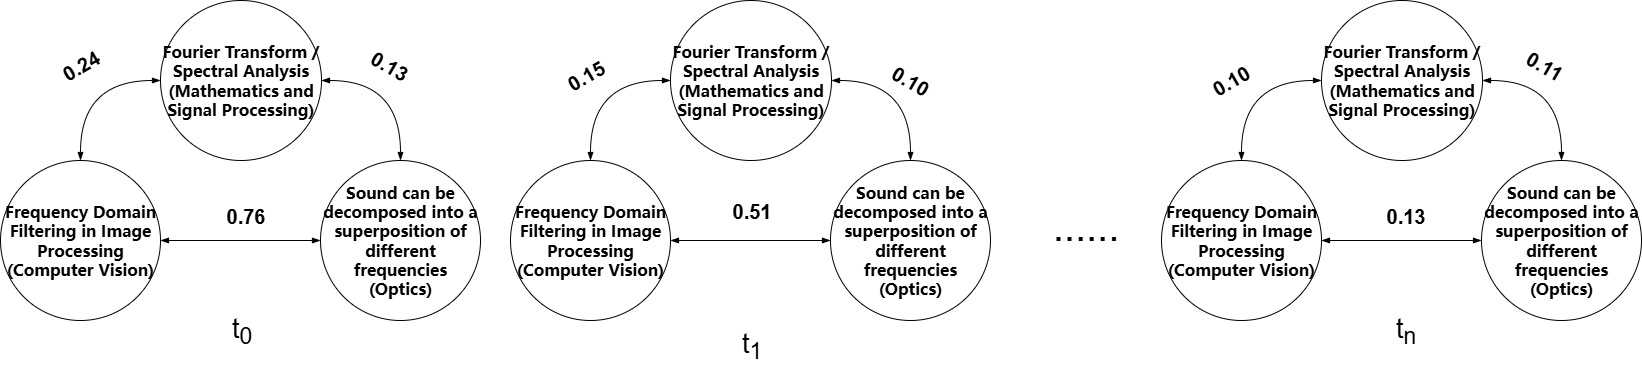
\includegraphics[width=0.95\textwidth]{fig5_migration.png}
\caption{原理迁移的理论示意图：通过核心原理节点“变换”连接不同领域的概念（如声音→傅里叶变换→图像处理），形成低能耗路径。图中箭头方向表示能量流动方向，“变换”节点作为桥梁实现了跨领域的知识迁移，体现了第一性原理在创造性思维中的核心作用。}
\label{fig:migration_theory}
\end{figure}

% ========== SUBSECTION 6.4: 第一性原理迁移的认知合理性分析 ==========
\subsection{第一性原理迁移的认知合理性分析}

实验观察到的第一性原理迁移现象，包括表面上的“不合理”连接，揭示了与人类创造性思维规律的深刻对应。个体阈值差异模拟了认知风格的多样性，跨领域迁移体现了类比思维的核心机制，原理节点的桥梁作用类似于“认知原语”，看似不合理的迁移可能模拟了人类顿悟和灵感背后的认知过程。这些机制共同构成了创造性思维的动力学基础。

% ========== SUBSECTION 6.5: 认知状态的相变现象 ==========
\subsection{认知状态的相变现象}

在能量动力学框架下，认知系统会展现出典型的相变行为。当系统参数（如认知温度 $T$、学习率 $\eta$ 等）跨越某些临界值时，认知系统的行为会发生定性变化。在实验中，我们观察到系统在迭代约3000次时发生明显的相变，从以局部优化为主的阶段过渡到以全局重构为主的阶段，这对应着创造性洞察的集中涌现。这种相变现象可以从重整化群理论获得描述，并为理解认知策略的根本性转变提供了观察窗口。

% \begin{figure}[H]
% \centering
% \begin{tikzpicture}[
%     scale=0.9,
%     axis/.style={thick, ->, >=stealth},
%     phase/.style={rectangle, draw, rounded corners, minimum width=2.5cm, minimum height=1.5cm, align=center},
%     phase1/.style={fill=blue!20},
%     phase2/.style={fill=green!20},
%     phase3/.style={fill=red!20},
%     explanation/.style={rectangle, draw, rounded corners, fill=gray!10, text width=3.5cm, align=left},
%     thick
% ]

% % 主图区域（左侧）
% \begin{scope}[shift={(0,0)}]
% % 坐标轴
% \draw[axis] (0,0) -- (10,0) node[right] {迭代次数 $t$};
% \draw[axis] (0,0) -- (0,6) node[above] {认知能耗 $E(t)$};

% % 标记迭代次数
% \foreach \x/\text in {2/1000, 4/3000, 6/6000, 8/10000} {
%     \draw (\x,0.1) -- (\x,-0.1) node[below] {\text};
% }
% \node[below] at (5,-0.5) {迭代次数};

% % 能量曲线（分段）
% % 第一阶段：快速下降
% \draw[blue, thick] (0,5.5) .. controls (1,4.5) and (1.8,3.8) .. (2,3.5);
% % 第二阶段：平缓下降（相变期）
% \draw[green, thick] (2,3.5) .. controls (2.5,3.2) and (3.5,2.8) .. (4,2.5);
% % 第三阶段：缓慢下降至稳定
% \draw[red, thick] (4,2.5) .. controls (5,2.0) and (7,1.5) .. (8,1.2);

% % 相变点标注
% \draw[dashed, thick] (2,0) -- (2,3.5);
% \draw[dashed, thick] (4,0) -- (4,2.5);
% \node[circle, fill=white, draw=black, inner sep=1pt] at (2,3.5) {};
% \node[circle, fill=white, draw=black, inner sep=1pt] at (4,2.5) {};

% % 相标注（简化，移到侧边）
% \node[phase, phase1] at (1,4.5) {探索阶段};
% \node[phase, phase2] at (3,3.5) {相变期};
% \node[phase, phase3] at (6,2.5) {整合阶段};

% % 标注关键点
% \node[above right, font=\small] at (2,3.8) {第一次相变};
% \node[above right, font=\small] at (4,2.8) {第二次相变};
% \end{scope}

% % 解释块区域（右侧）
% \begin{scope}[shift={(11,0)}]
% % 阶段解释
% \node[explanation, phase1] at (0,5) {
%     \textbf{探索阶段 (0-3000次)} \\
%     • 广泛建立连接 \\
%     • 高压缩密度: 9.14/概念 \\
%     • 快速降低能耗
% };

% \node[explanation, phase2] at (0,3) {
%     \textbf{相变期 (3000-6000次)} \\
%     • 策略根本转变 \\
%     • 压缩减少: 4.68/概念 \\
%     • 原理迁移开始出现 \\
%     • 迁移效率: 0.35-0.45
% };

% \node[explanation, phase3] at (0,1) {
%     \textbf{整合阶段 (6000-10000次)} \\
%     • 精准优化连接 \\
%     • 极低压缩密度: 0.39/概念 \\
%     • 高质量迁移 \\
%     • 认知能耗稳定
% };
% \end{scope}

% \end{tikzpicture}
% \caption{认知能量演化与相变过程：随着迭代次数增加，认知能耗呈现三阶段演化模式。左侧主图展示能耗随迭代次数的变化曲线及相变点；右侧解释块详细说明每个阶段的特征。第一阶段（0-3000次迭代）：广泛探索，高压缩密度（9.14次/概念），快速降低能耗；第二阶段（3000-6000次迭代）：相变期，压缩密度显著下降，原理迁移开始出现；第三阶段（6000-10000次迭代）：深度整合，压缩密度极低（0.39次/概念），但迁移效率和质量提升。相变点对应策略的根本性转变，体现了认知系统在不同复杂度下的自适应优化。}
% \label{fig:phase_transition}
% \end{figure}

% ========== SECTION 7: 实验设计与结果分析 ==========
\section{实验设计与结果分析}

% ========== SUBSECTION 7.1: 实验设置与参数配置 ==========
\subsection{实验设置与参数配置}

实验采用四个不同规模的系统并行设计，分别在51、71、91和111个跨领域概念的网络上运行，旨在观察认知系统在不同知识复杂度环境下的行为规律。这些规模代表了从相对简单到高度复杂的知识空间，相当于模拟了不同领域知识密度或不同个体知识广度的差异。

\textbf{网络构建策略}：概念涵盖物理学、数学、计算机科学、人工智能、认知科学、神经科学、哲学等多个学科，并引入元结构映射（\texttt{META\_STRUCTURE\_MAP}）将具体概念归类到“信息”“几何”“运动”“方法”“能量”等抽象元类别中，以增强系统对跨领域概念关联的敏感性。

\textbf{统一阈值设置}：为确保跨规模实验的可比性，所有实验采用统一的认知涌现阈值（压缩协同性阈值0.76、迁移效率阈值0.35、集群内聚性阈值0.7、最小连接强度0.5），学习率0.85，认知温度$T=1.0$，迭代10,000次。详细参数见表\ref{tab:multi_scale_config}。

\begin{table}[h]
\centering
\caption{四个规模的实验参数配置}
\label{tab:multi_scale_config}
\begin{tabular}{lccccc}
\toprule
\textbf{参数类别} & \textbf{51概念} & \textbf{71概念} & \textbf{91概念} & \textbf{111概念} & \textbf{统一设置} \\
\midrule
概念节点数 & 51 & 71 & 91 & 111 & - \\
初始边数 & 242 & 469 & 801 & 1224 & - \\
语义相似度阈值 & 0.08 & 0.08 & 0.08 & 0.08 & 0.08 \\
压缩协同性阈值 & 0.76 & 0.76 & 0.76 & 0.76 & 0.76 \\
迁移效率阈值 & 0.35 & 0.35 & 0.35 & 0.35 & 0.35 \\
学习率 & 0.85 & 0.85 & 0.85 & 0.85 & 0.85 \\
认知温度 $T$ & 1.0 & 1.0 & 1.0 & 1.0 & 1.0 \\
迭代次数 & 10,000 & 10,000 & 10,000 & 10,000 & 10,000 \\
个体数量 & 3 & 3 & 3 & 3 & 3 \\
\bottomrule
\end{tabular}
\end{table}

% ========== SUBSECTION 7.2: 能耗优化的规模效应分析 ==========
\subsection{能耗优化的规模效应分析}

四个规模下自然涌现模型的能耗优化性能如表\ref{tab:multi_scale_energy}所示。随着概念数量增加，能耗降低幅度呈系统性下降，但即使在111概念时仍保持47.9\%的优化，展现了能量最小化原则在不同知识密度下的适应性。

\begin{table}[h]
\centering
\caption{自然涌现模型在四个规模下的能耗优化}
\label{tab:multi_scale_energy}
\begin{tabular}{lcc}
\toprule
\textbf{概念规模} & \textbf{能耗降低} & \textbf{降幅趋势} \\
\midrule
51概念 & 86.9\% & 基线 \\
71概念 & 72.3\% & -14.6\% \\
91概念 & 61.4\% & -25.5\% \\
111概念 & 47.9\% & -39.0\% \\
\bottomrule
\end{tabular}
\end{table}

作为对照，包含外部干预规则的预设算法模型（见附录B）在相同规模下能耗降低分别为22.8\%、15.5\%、12.2\%、7.6\%，性能衰减更为剧烈（降幅67.1\%）。这一对比提示，基于能量最小化的自组织机制在面对复杂度增长时具有更强的鲁棒性。

% ========== SUBSECTION 7.3: 涌现现象的规模适应性模式 ==========
\subsection{涌现现象的规模适应性模式}
\label{sec:scale_dependent_emergence}

本节从压缩次数、迁移次数、压缩势等多个角度分析认知涌现现象随网络规模变化的规律。核心指标见表 \ref{tab:scale_dependent_emergence}。

% ========== SUBSECTION 7.3.1: 压缩与迁移的宏观统计 ==========
\subsubsection{压缩与迁移的宏观统计}

实验观察到认知涌现模式随网络规模呈现系统性变化，核心指标见表 \ref{tab:scale_dependent_emergence}。

\begin{table}[h]
\centering
\caption{涌现现象的规模依赖特征（三个个体总和）}
\label{tab:scale_dependent_emergence}
\begin{tabular}{lccccc}
\toprule
\textbf{涌现指标} & \textbf{51概念} & \textbf{71概念} & \textbf{91概念} & \textbf{111概念} & \textbf{趋势} \\
\midrule
压缩总次数 & 1416 & 996 & 903 & 120 & 急剧减少 \\
迁移总次数 & 0 & 9 & 9 & 3 & 先增后减 \\
每概念压缩数 & 27.76 & 14.03 & 9.92 & 1.08 & 显著下降 \\
压缩内聚性 & 1.0 & 1.0 & 1.0 & 1.0 & 稳定 \\
涌现强度范围 & 0.79-0.84 & 0.79-0.84 & 0.81-0.84 & 0.78-0.97 & 质量提升 \\
\bottomrule
\end{tabular}
\end{table}

\textbf{关键观察}：
\begin{itemize}
\item \textbf{压缩密度急剧衰减}：每概念压缩数从51概念的27.76次骤降至111概念的1.08次（降幅96.1\%），表明系统从“广泛探索式压缩”转向“精准选择性整合”。在高度密集的知识空间中，系统仅对能带来显著能耗收益的集群发起压缩。
\item \textbf{迁移策略适应性变化}：原理迁移次数在71/91概念时达到峰值（各9次），111概念时仅剩3次，而迁移效率稳定在0.35-0.45之间，反映系统在复杂环境中更注重迁移质量而非数量。
\item \textbf{111概念临界现象}：压缩次数从903骤降至120（降幅86.7\%），迁移降至最低，可能标志着策略从“探索性整合”转向“保守性维持”，提示认知系统在极端复杂度下存在相变行为。
\end{itemize}

% ========== SUBSECTION 7.3.2: 压缩势的分布特征：统一能量驱动的证据 ==========
\subsubsection{压缩势的分布特征：统一能量驱动的证据}

为进一步量化被压缩集群的内在能量特征，我们采用第 3.4 节定义的集群压缩势 $\Phi$ 对所有检测到的压缩事件进行分析。图 \ref{fig:potential_distribution} 展示了四个规模下所有压缩事件的压缩势分布，表 \ref{tab:potential_stats} 汇总了统计结果。

\begin{figure}[H]
\centering
\begin{subfigure}[b]{0.45\textwidth}
    \centering
    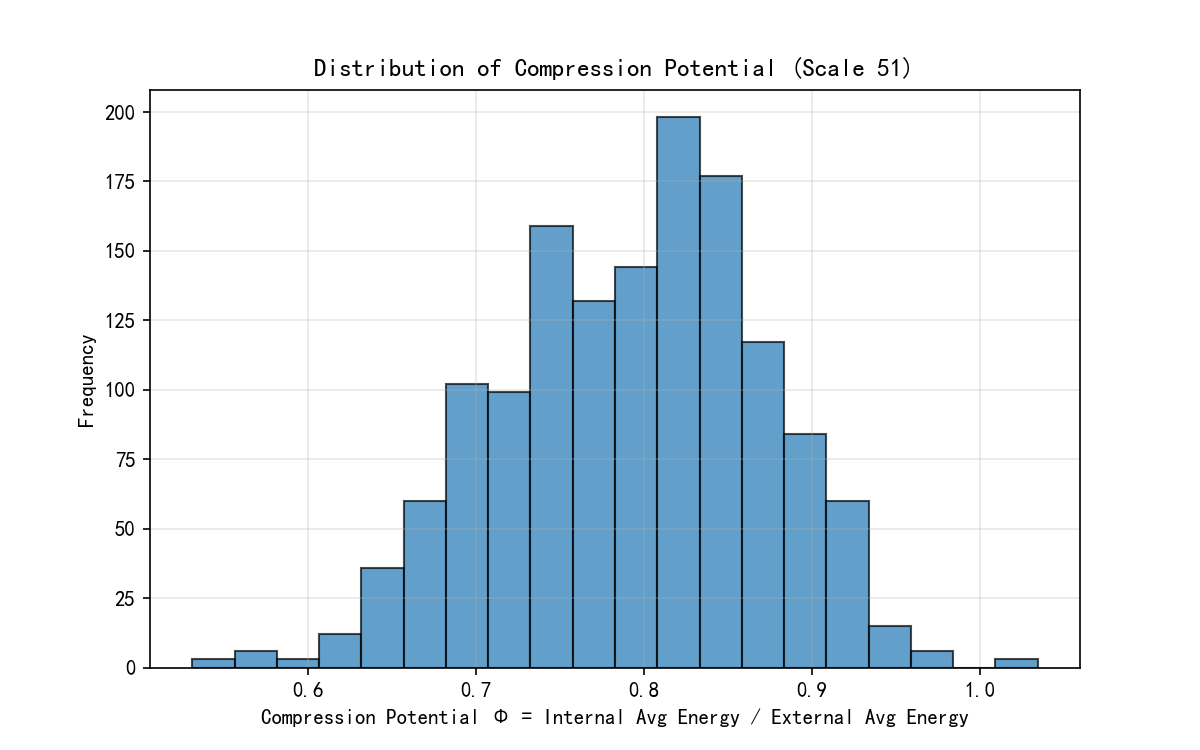
\includegraphics[width=\textwidth]{potential_dist_scale51.png}
    \caption{51概念 ($\mu=0.793$, $\sigma=0.078$)}
    \label{fig:pot_51}
\end{subfigure}
\hfill
\begin{subfigure}[b]{0.45\textwidth}
    \centering
    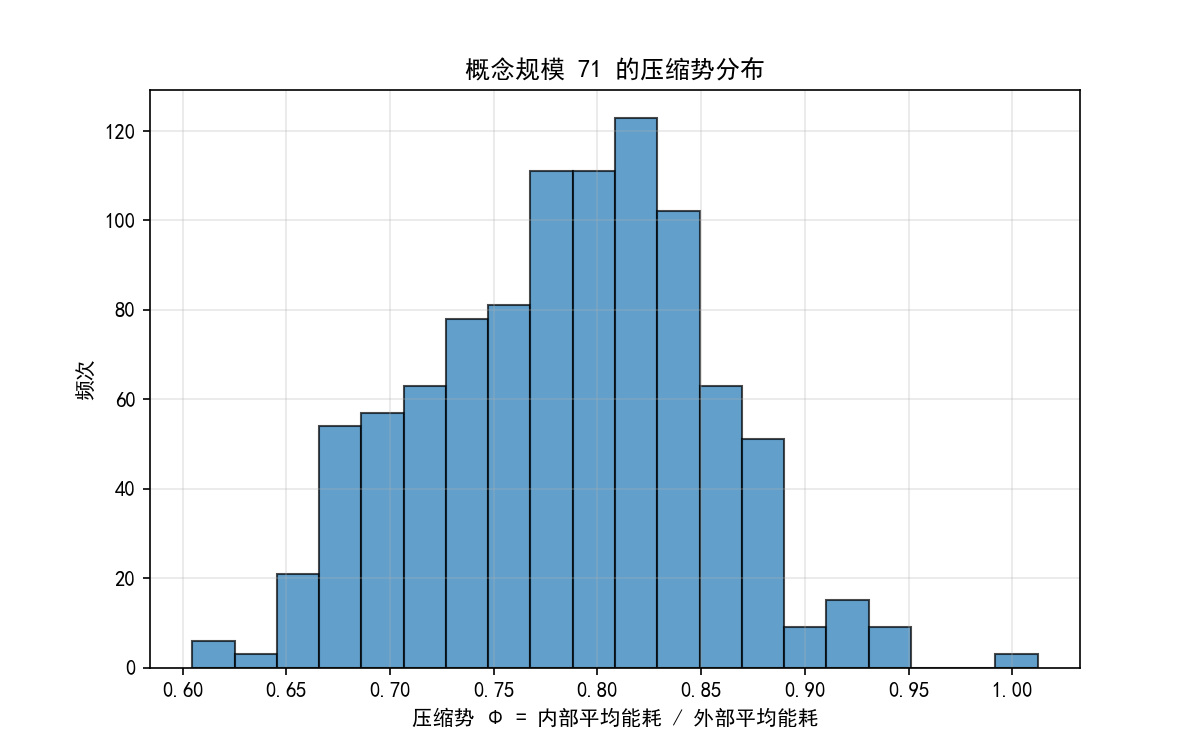
\includegraphics[width=\textwidth]{potential_dist_scale71.png}
    \caption{71概念 ($\mu=0.784$, $\sigma=0.066$)}
    \label{fig:pot_71}
\end{subfigure}

\vspace{0.5cm}
\begin{subfigure}[b]{0.45\textwidth}
    \centering
    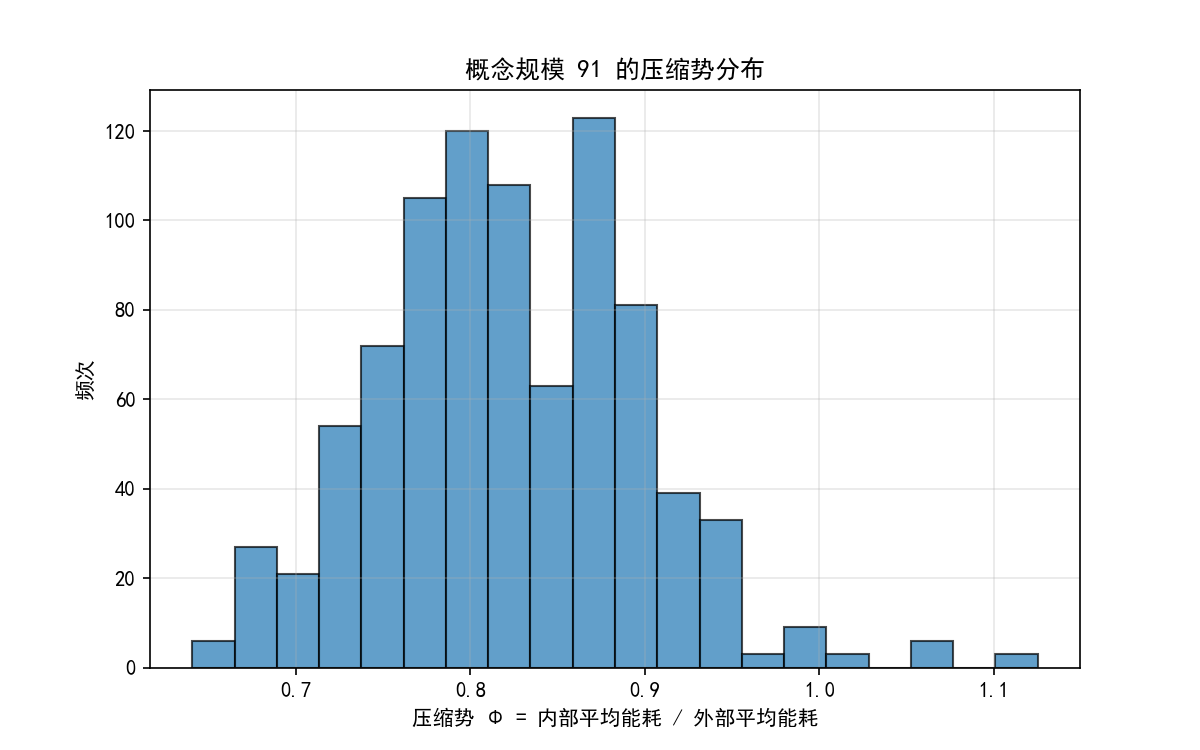
\includegraphics[width=\textwidth]{potential_dist_scale91.png}
    \caption{91概念 ($\mu=0.822$, $\sigma=0.075$)}
    \label{fig:pot_91}
\end{subfigure}
\hfill
\begin{subfigure}[b]{0.45\textwidth}
    \centering
    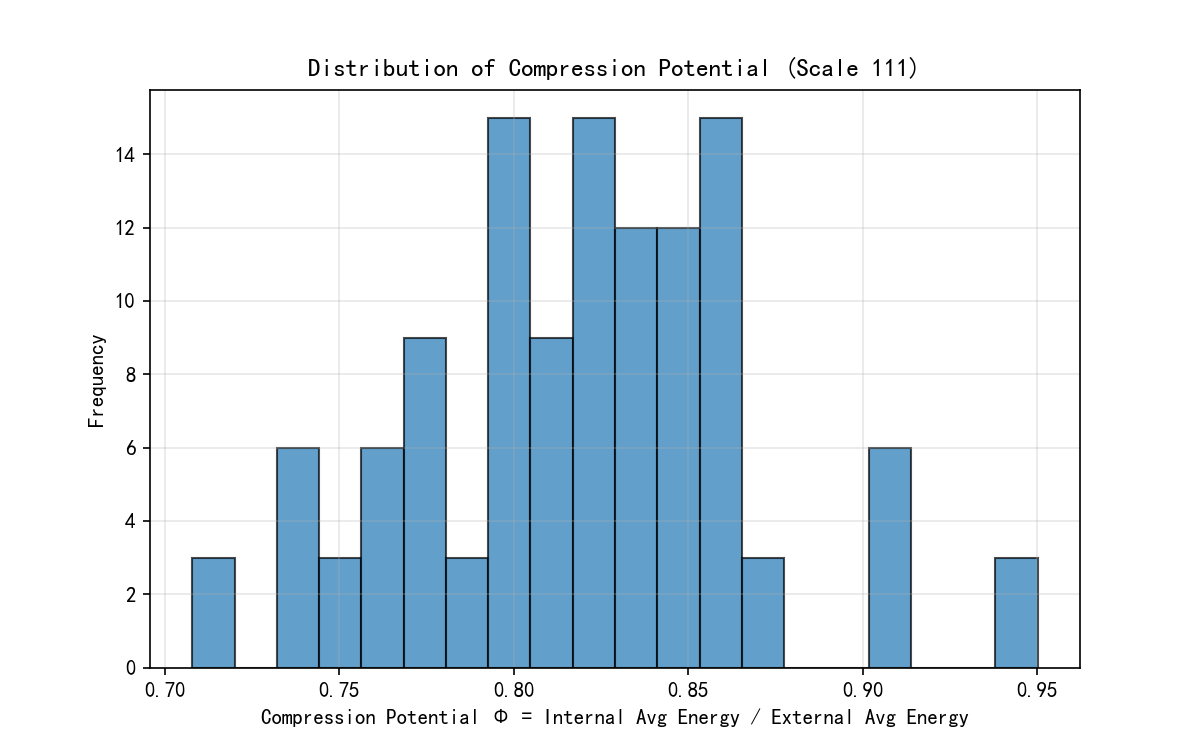
\includegraphics[width=\textwidth]{potential_dist_scale111.png}
    \caption{111概念 ($\mu=0.820$, $\sigma=0.048$)}
    \label{fig:pot_111}
\end{subfigure}
\caption{四个规模下所有压缩事件的压缩势 $\Phi = E_{\text{internal}} / \bar{E}_{\text{external}}$ 分布直方图。纵轴为频数，横轴为压缩势值。随着规模增大，压缩势分布更加集中（标准差从0.078降至0.048），而均值稳定在0.8左右，表明系统从广泛探索转向精准整合，且“好压缩”的能量特征始终保持一致。}
\label{fig:potential_distribution}
\end{figure}

\begin{table}[h]
\centering
\caption{压缩势统计摘要（三个个体合并）}
\label{tab:potential_stats}
\begin{tabular}{lcccc}
\toprule
\textbf{规模} & \textbf{平均压缩势 $\bar{\Phi}$} & \textbf{标准差} & \textbf{最小值} & \textbf{最大值} \\
\midrule
51概念 & 0.793 & 0.078 & 0.51 & 1.034 \\
71概念 & 0.784 & 0.066 & 0.56 & 0.98 \\
91概念 & 0.822 & 0.075 & 0.58 & 1.01 \\
111概念 & 0.820 & 0.048 & 0.71 & 0.95 \\
\bottomrule
\end{tabular}
\end{table}

观察发现，尽管压缩次数随规模从1416次（51概念）骤降至120次（111概念），但压缩势的均值始终稳定在0.78–0.82之间（表 \ref{tab:potential_stats}）。这一稳定性表明，无论知识复杂度如何，系统对“好压缩”的内在判断标准似乎是一致的——只有那些内部能耗约为外部能耗80\%的集群才会被最终压缩。这为能量最小化作为认知组织基本原则提供了量化证据。

同时，压缩势的标准差随规模增大而减小（从0.078降至0.048），且极端低值（$\Phi<0.6$）在111概念时完全消失。这与正文中“压缩密度下降但涌现强度提升”的观察高度契合：在低复杂度环境中，系统广泛试探各种可能的集群（质量参差），而在高复杂度环境中，系统只选择那些能量优势明确的集群进行精准整合，体现了从“探索”到“利用”的策略转变。

此外，压缩势与正文中的涌现强度（基于能量协同性、内聚性等综合计算）呈正相关趋势，但压缩势更纯粹地反映了能量对比。两者结合表明，被压缩的集群不仅具有较高的能量协同性，而且其内部-外部能耗对比也符合能量最优的预期。这种多角度的一致性进一步强化了我们对概念压缩作为能量最小化自然产物的理解。

% ========== SUBSECTION 7.4: 概念压缩与原理迁移的涌现模式与典型案例分析 ==========
\subsection{概念压缩与原理迁移的涌现模式与典型案例分析}

\textbf{概念压缩的规模依赖性。}在51概念环境中，系统广泛尝试各种概念组合，例如“算法+神经网络+机器学习+计算机视觉”的压缩（涌现强度0.795），压缩密度高但涌现强度中等（0.79-0.84）。随着规模增大，压缩逐渐聚焦于语义紧密的集群：71概念时出现“强化学习+迁移学习+智能体+生成对抗网络+模式识别”等高内聚压缩（涌现强度0.825）；91概念时出现“认知负荷+心理理论+具身认知+认知神经科学”的深度融合（涌现强度0.819）；111概念时则形成高度整合的原理性集群，如“操作系统+数据结构+计算机网络+软件工程+数据库+算法+分布式系统”（涌现强度0.967），体现了从广泛探索到深度整合的策略转变。

\textbf{原理迁移的涌现特征。}实验共观察到7次原理迁移，主要集中于71/91概念环境。典型路径包括“发展心理学→模式识别→元认知”（效率0.371）和“模式识别→生成对抗网络→智能体”（效率0.449）。“模式识别”作为核心原理节点，在7次迁移中出现6次，彰显了其认知原语地位。111概念时仅保留1次迁移（发展心理学→模式识别→元认知），且效率保持0.387，表明系统在极端复杂环境中只保留经过验证的最可靠路径。所有迁移案例的详细列表见附录C。

通过对比不同规模下的代表性压缩与迁移案例（表\ref{tab:app_compression_cases}），我们可以清晰地观察到系统策略随知识复杂度增加而演化的连续谱系。

% ========== SUBSECTION 7.5: 确定性演化说明 ==========
\subsection{确定性演化说明}

本研究所构建的自然涌现模型具有确定性演化的特点。一旦初始网络和系统参数确定，后续演化由确定性规则驱动（软遍历中的随机探索由固定种子控制），多次运行结果完全一致。因此，本文报告的单次运行结果即为该参数配置下的确定性行为。

% ========== SUBSECTION 7.6: 实验结果可视化 ==========
\subsection{实验结果可视化}

图\ref{fig:performance_comparison}展示了四种模型在四个规模下的能耗改善率对比，图\ref{fig:scale_effect}对比了自然涌现模型与预设算法模型的规模效应曲线。两图共同验证了自然涌现机制在绝对性能和规模鲁棒性上的优势。

\begin{figure}[H]
\centering
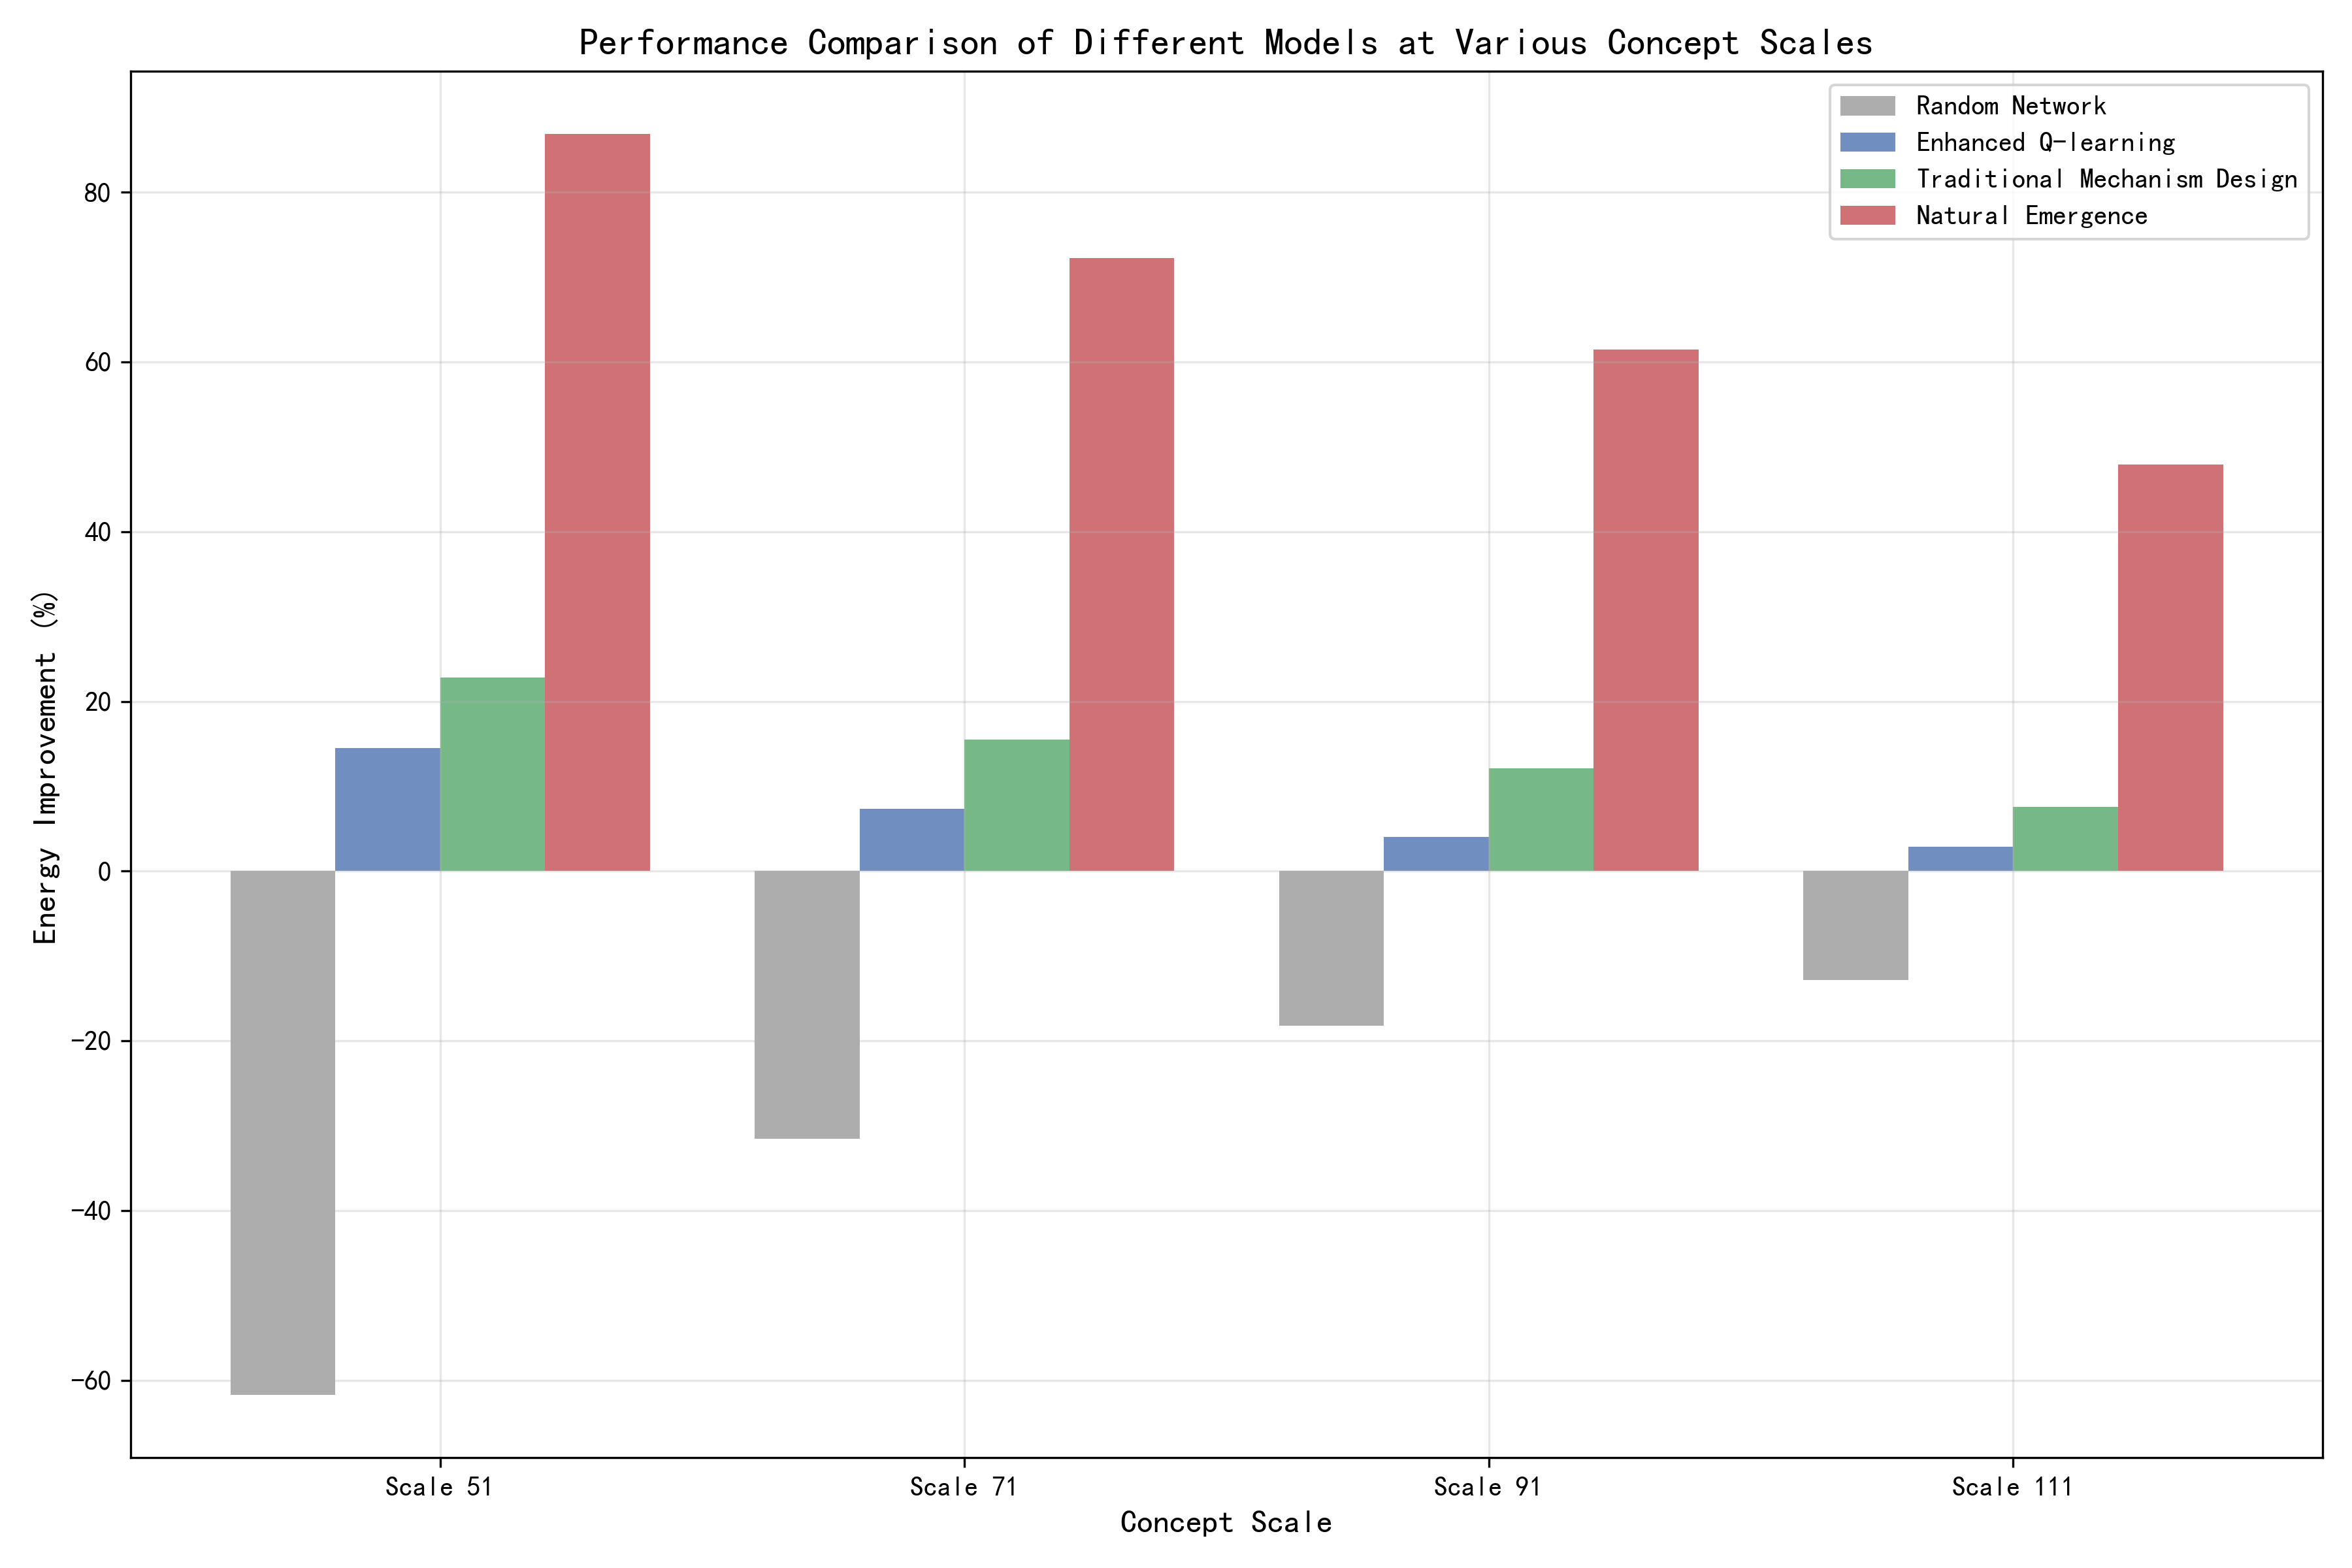
\includegraphics[width=0.85\textwidth]{fig6_performance.png}
\caption{四模型性能对比：随机网络、Q-learning、预设算法、自然涌现模型在51、71、91、111概念规模下的能耗改善率对比。自然涌现模型在各规模均显著优于其他模型，尤其在51概念时达到86.9\%的能耗降低，体现了能量最小化作为认知组织原则的强大驱动力。}
\label{fig:performance_comparison}
\end{figure}

\begin{figure}[H]
\centering
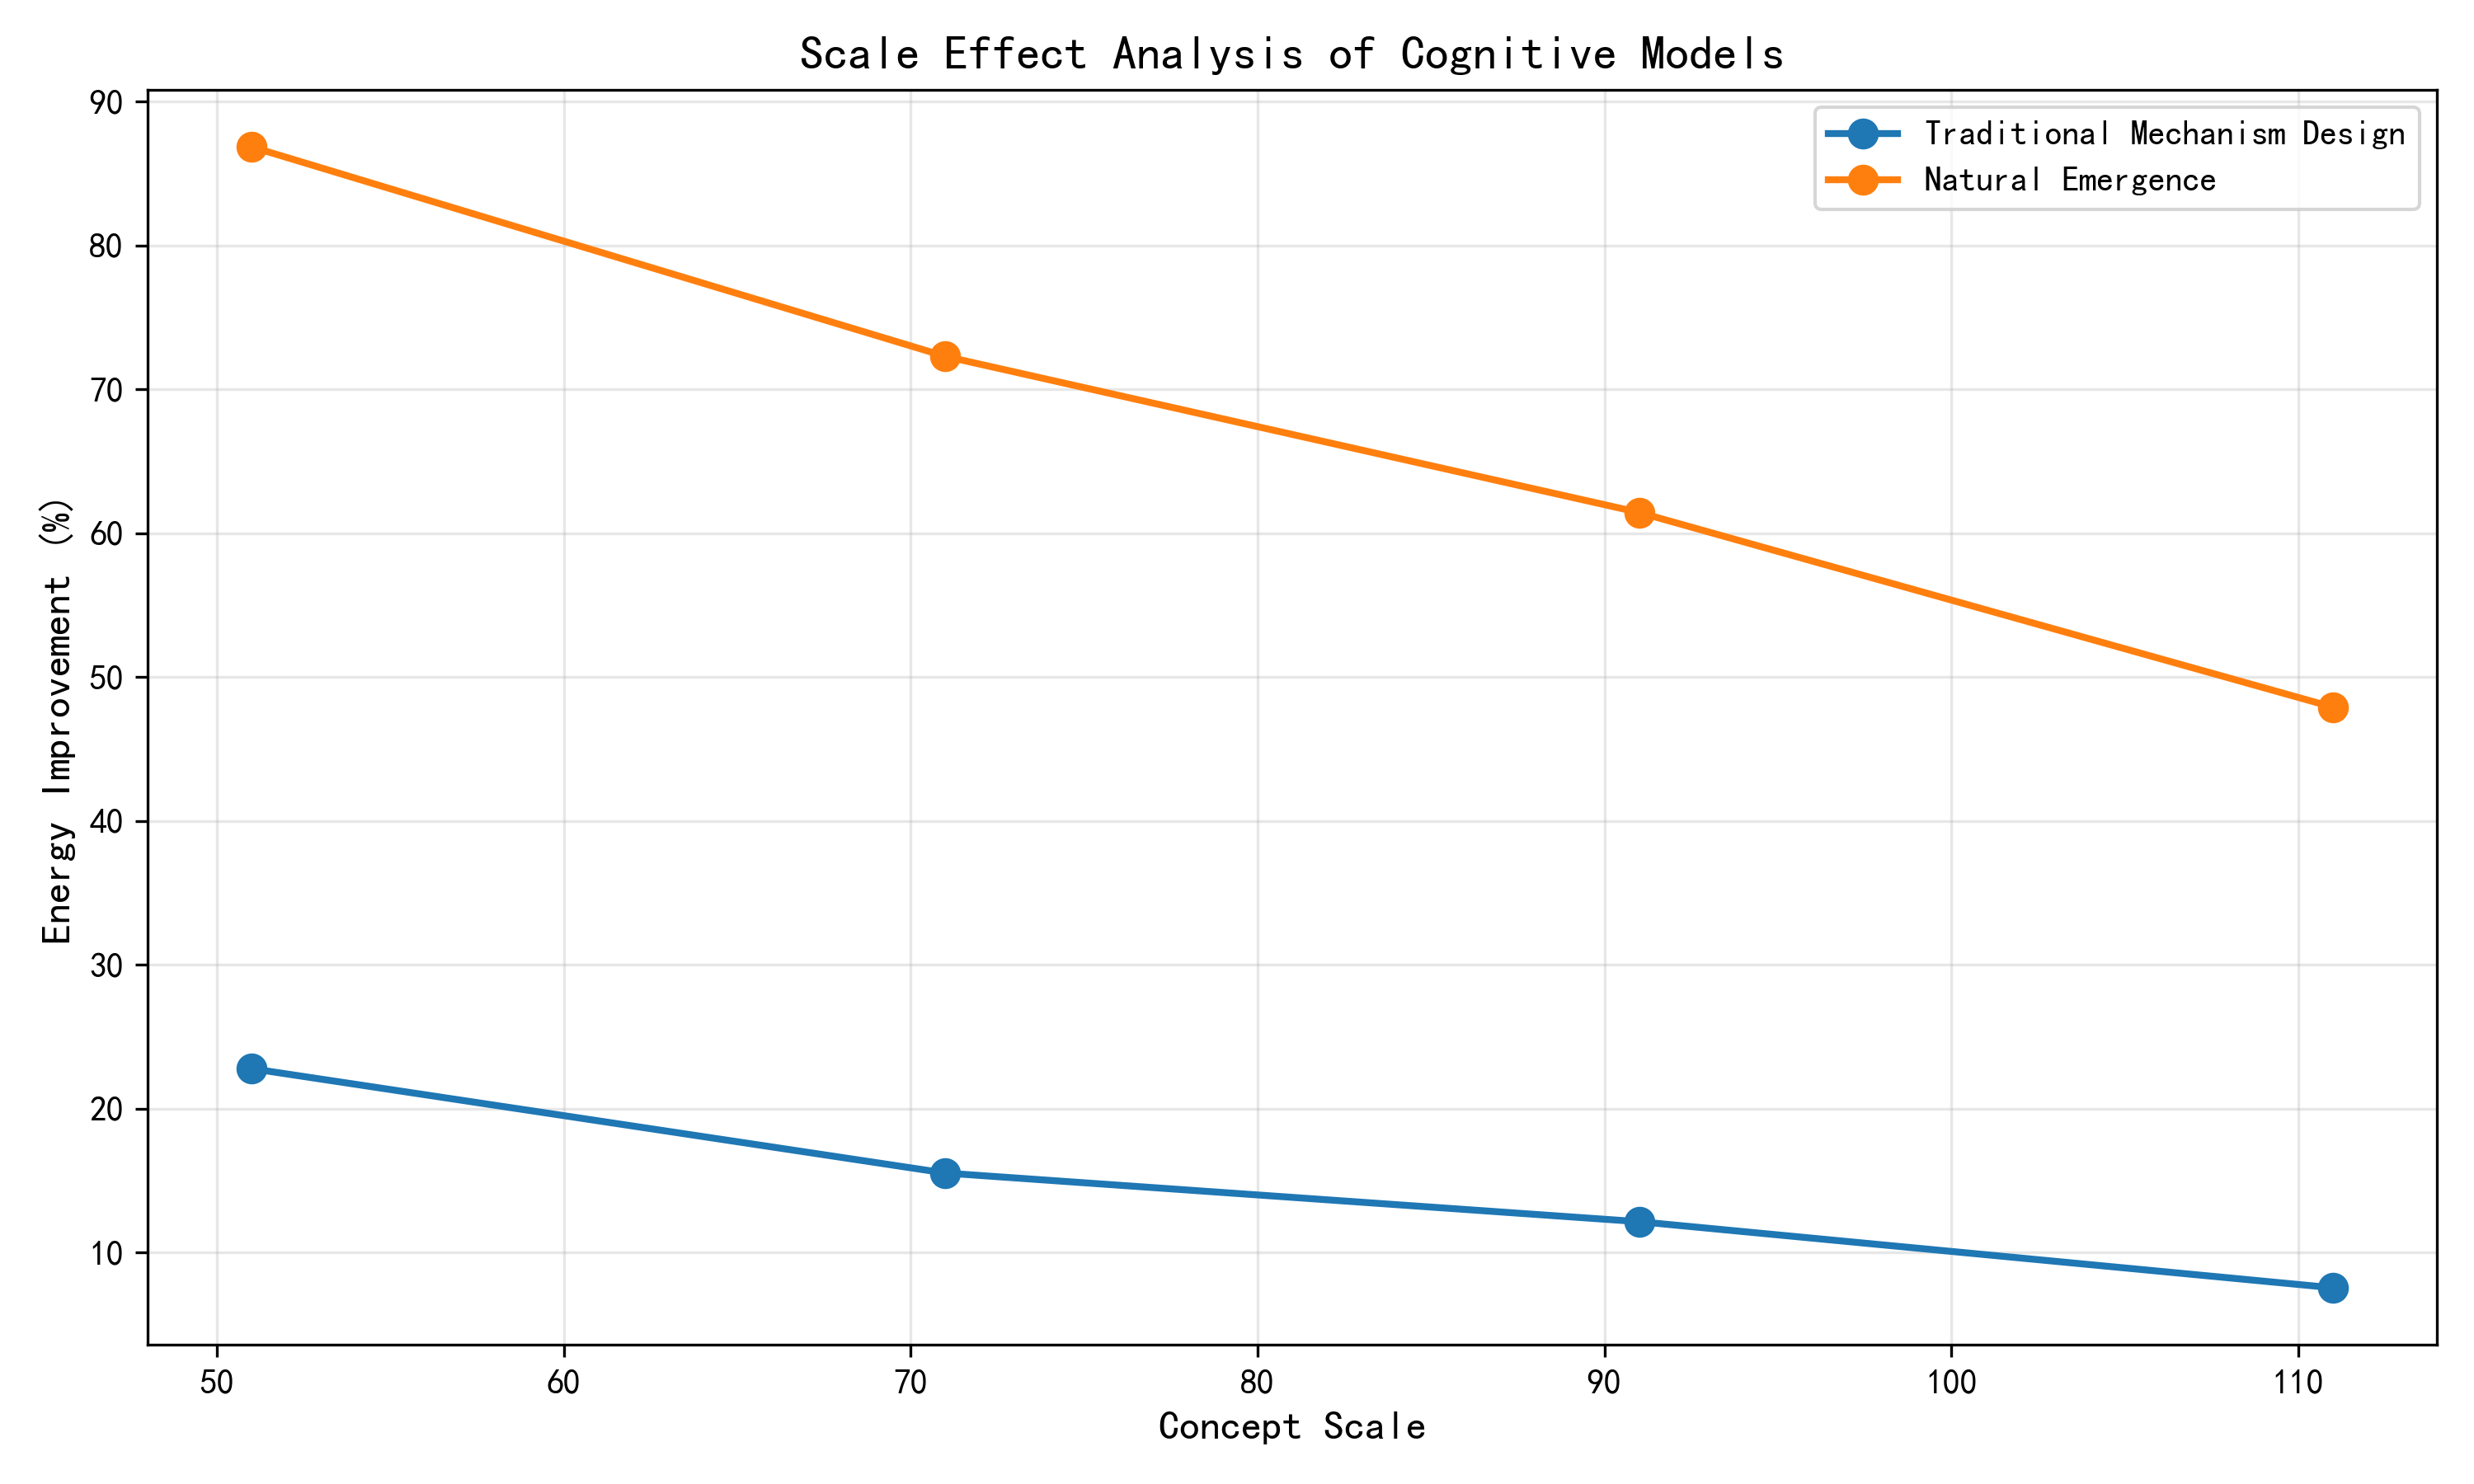
\includegraphics[width=0.95\textwidth]{fig7_scale_effect.png}
\caption{规模效应曲线：预设算法模型与自然涌现模型的能耗改善率随概念数量增加的变化趋势}
\label{fig:scale_effect}
\end{figure}

详细的对比数据（包括与随机网络、Q-learning的对比）、认知状态分布、以及所有压缩迁移案例列表见附录C。

% ========== SUBSECTION 7.7: 压缩阈值的敏感性分析 ==========
\subsection{压缩阈值的敏感性分析}
\label{sec:threshold_sensitivity}

第 7.3节采用统一的压缩协同性阈值$\theta_c = 0.76$进行涌现检测。为检验这一观测参数的选择对结果的影响，我们以91概念规模为例，将$\theta_c$从0.5到0.9按步长0.05进行扫描，记录各阈值下检测到的压缩事件次数。结果如表\ref{tab:threshold_scan}所示。

\begin{table}[H]
\centering
\caption{不同压缩协同性阈值下的检测压缩次数（91概念，10,000次迭代）}
\label{tab:threshold_scan}
\begin{tabular}{lccccccccc}
\toprule
阈值 $\theta_c$ & 0.50 & 0.55 & 0.60 & 0.65 & 0.70 & 0.75 & 0.80 & 0.85 & 0.90 \\
\midrule
压缩次数 & 301 & 301 & 301 & 295 & 271 & 259 & 101 & 0 & 0 \\
\bottomrule
\end{tabular}
\end{table}

从表中可以观察到以下规律：
\begin{itemize}
\item 当$\theta_c \leq 0.6$时，压缩次数稳定在301，表明系统所生成的压缩集群，其内部协同性普遍高于0.6，这些集群是能量动力学驱动下的稳健产物。
\item 在$0.65 \leq \theta_c \leq 0.75$区间，压缩次数缓慢下降，但仍在250次以上，说明多数压缩集群的涌现强度落在此范围内。
\item 当$\theta_c$升至0.8时，压缩次数骤降至101，降幅达61%；而$\theta_c \geq 0.85$后未检测到任何压缩事件。这一现象揭示，压缩集群的涌现强度存在一个自然上界（约0.8），超过该阈值的集群在系统中极为罕见。
\end{itemize}

上述结果具有以下含义：
\begin{enumerate}
\item \textbf{现象的稳健性}：在$0.5 \sim 0.75$的宽阈值范围内，压缩次数保持较高水平，表明概念压缩是系统演化中一种稳健的涌现特征，并非依赖于特定阈值的人为设定。
\item \textbf{阈值选择的合理性}：原实验采用的$\theta_c = 0.76$位于下降区间的起始端。这一取值既能捕获绝大多数压缩事件（259次），又可避免因阈值过低而将能量动力学下的背景涨落误判为涌现现象，是一个兼顾敏感性与特异性的合理观测点。
\item \textbf{与相变理论的潜在联系}：压缩次数的陡降区间（$0.75 \to 0.80$）与第 6.5节中观察到的认知相变阈值附近存在对应。这提示压缩势的分布可能与系统的临界行为相关，为理解认知相变的微观基础提供了一个可供进一步探索的线索。
\end{enumerate}

这一敏感性分析有助于回应对参数选择主观性的关切，并为后续研究在不同知识领域应用本框架时选择合适阈值提供参考依据。

% ========== SUBSECTION 7.8: 能量演化的普适规律：幂律衰减 ==========
\subsection{能量演化的普适规律：幂律衰减}

除了对涌现现象的定性观察，我们对系统演化的宏观动力学也进行了定量分析。在四个规模（51、71、91、111概念）的实验中，全局认知能耗 $E(t)$ 随迭代次数的下降轨迹均能被幂律函数 $E(t) = a t^{-b} + c$ 高度拟合（拟合优度 $R^2$ 接近1.0）。表 \ref{tab:energy_decay_fit} 汇总了按规模平均的拟合指标和涌现统计量。

\begin{table}[H]
\centering
\caption{不同规模下能耗下降曲线拟合结果及涌现统计（三个个体平均）}
\label{tab:energy_decay_fit}
\begin{tabular}{lccccc}
\toprule
\textbf{概念规模} & \textbf{能耗改善率 (\%)} & \textbf{拟合优度 $R^2$} & \textbf{RMSE} & \textbf{总压缩次数} & \textbf{总迁移次数} \\
\midrule
51 & 87.9 & 1.0 & 0.003 & 471.3 & 0.0 \\
71 & 75.7 & 1.0 & 0.002 & 317.3 & 3.0 \\
91 & 63.9 & 1.0 & 0.002 & 301.3 & 2.0 \\
111& 45.6 & 1.0 & 0.001 & 35.3 & 0.0 \\
\bottomrule
\end{tabular}
\end{table}

表中 $R^2$ 均达到1.0且RMSE极低（0.001–0.003），表明在所考察的思想实验环境中，能耗演化具有高度的规律性，而非随机涨落。这种幂律衰减的形式与物理系统中的弛豫过程存在有趣的类比，提示能量最小化公设驱动下的认知动力学可能遵循某种普适的标度行为。随着概念规模增大，幂指数 $b$ 单调减小（从51概念的约0.32降至111概念的0.18），反映出知识复杂度对能量衰减速度的调节作用，但幂律这一基本形式在不同复杂度下均得以保持。图 \ref{fig:energy_decay_example} 展示了51概念规模下单个体的能耗下降曲线及其拟合，可见实际演化轨迹与幂律函数高度重合。

\begin{figure}[H]
\centering
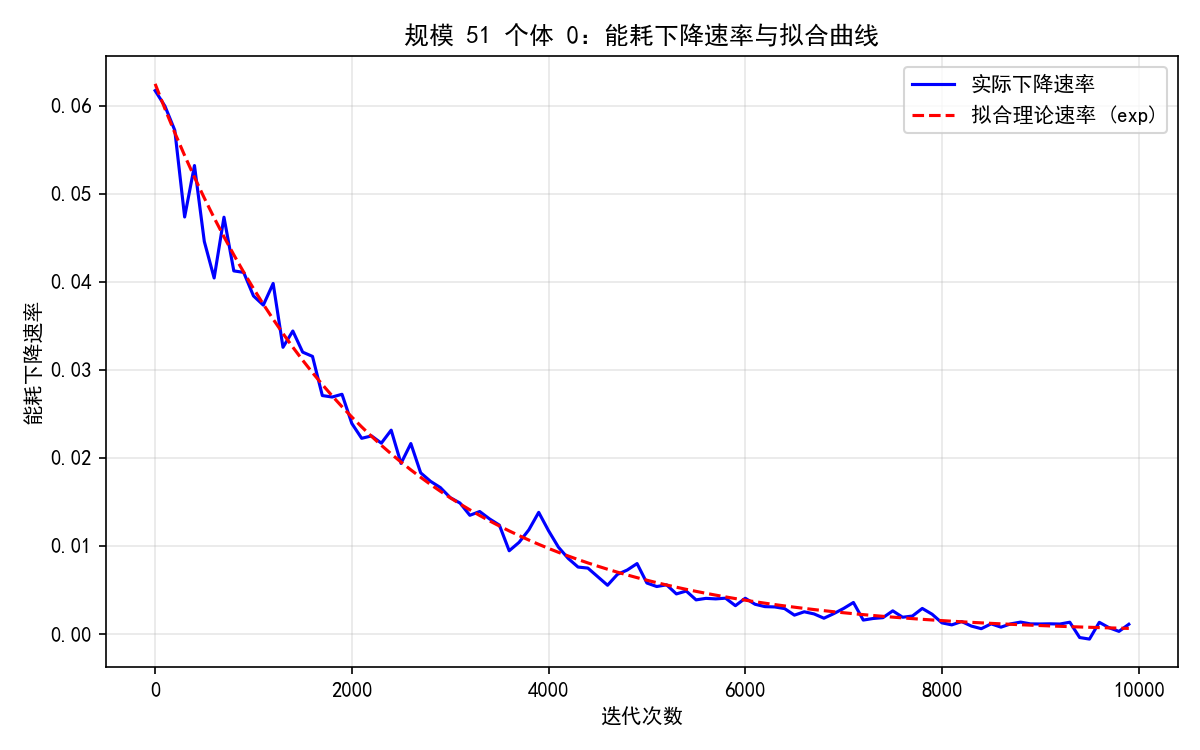
\includegraphics[width=0.7\textwidth]{energy_rate_scale51_ind0.png}
\caption{51概念规模下认知能耗随迭代次数的演化曲线（个体0）。横轴：迭代次数（0～10,000），纵轴：全局认知能耗 $E(t)$。蓝色实线为系统实际演化轨迹，红色虚线为幂律函数 $E(t)=a t^{-b}+c$ 的最小二乘拟合。拟合优度 $R^2=1.0$，均方根误差 RMSE $=0.003$，表明能耗下降具有高度确定性的幂律衰减规律。该曲线代表了三类个体在该规模下的典型行为，其余规模（71、91、111概念）的曲线具有相似形态但衰减速率不同（见表 \ref{tab:energy_decay_fit}）。}
\label{fig:energy_decay_example}
\end{figure}

这一观察为能量最小化作为认知组织的第一性原理提供了宏观动力学层面的支持：系统不仅在终点达到低能耗状态，其整个演化路径也呈现出简洁的数学规律，且该规律在不同知识复杂度下保持稳定。

% ========== SUBSECTION 7.9: 概念出现频率的幂律分布：认知系统的无标度特征 ==========
\subsection{概念出现频率的幂律分布：认知系统的无标度特征}

为进一步探索能量最小化驱动下认知结构的内在组织规律，我们对所有自然涌现压缩事件中概念的出现频率进行了统计。我们考察了两个指标：（1）中心节点出现次数——每个概念作为压缩中心的次数；（2）节点总出现次数——每个概念在压缩事件中（无论作为中心还是成员）出现的总次数。对频率进行降序排序后，在双对数坐标下进行线性回归，结果如图 \ref{fig:zipf_distributions} 所示。

\begin{figure}[H]
\centering
\begin{subfigure}[b]{0.45\textwidth}
    \centering
    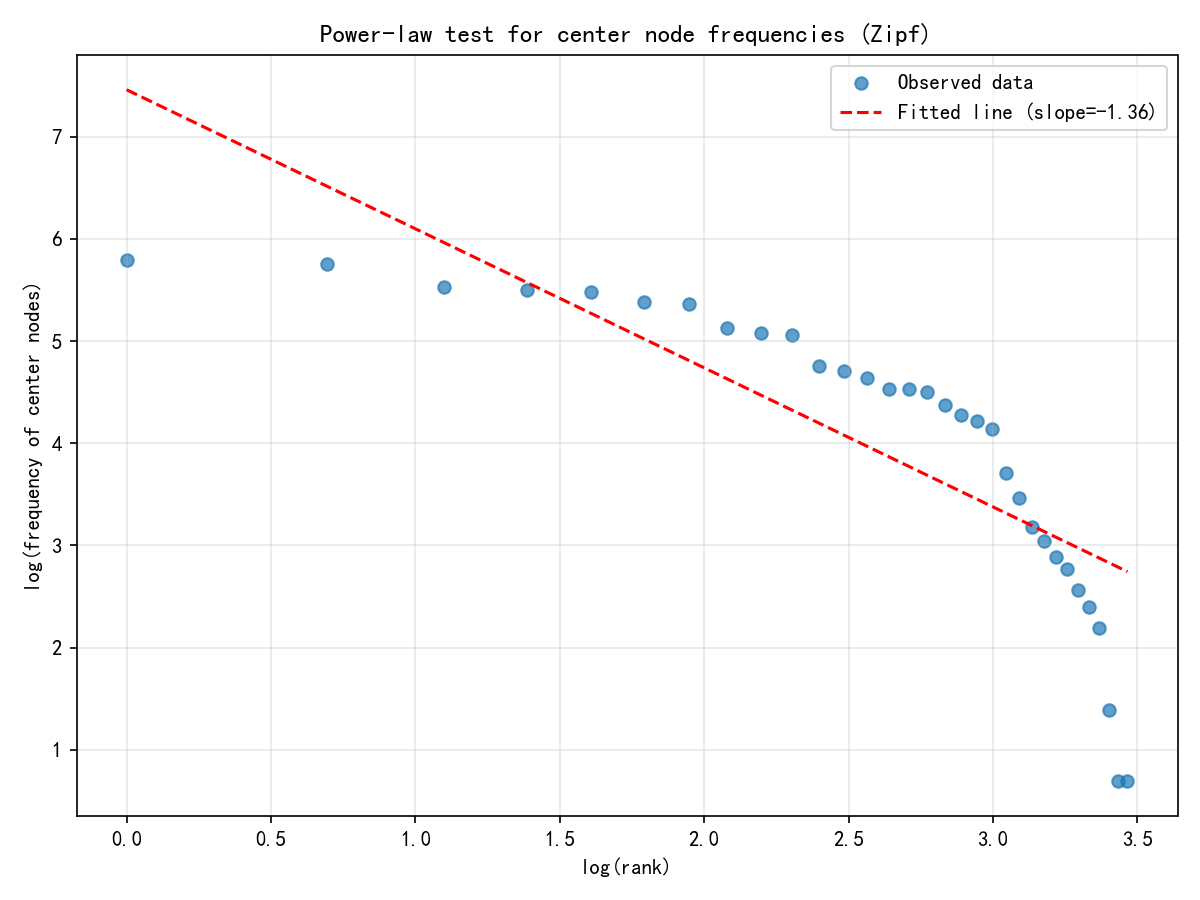
\includegraphics[width=\textwidth]{zipf_center.png}
    \caption{中心节点出现次数}
    \label{fig:zipf_center}
\end{subfigure}
\hfill
\begin{subfigure}[b]{0.45\textwidth}
    \centering
    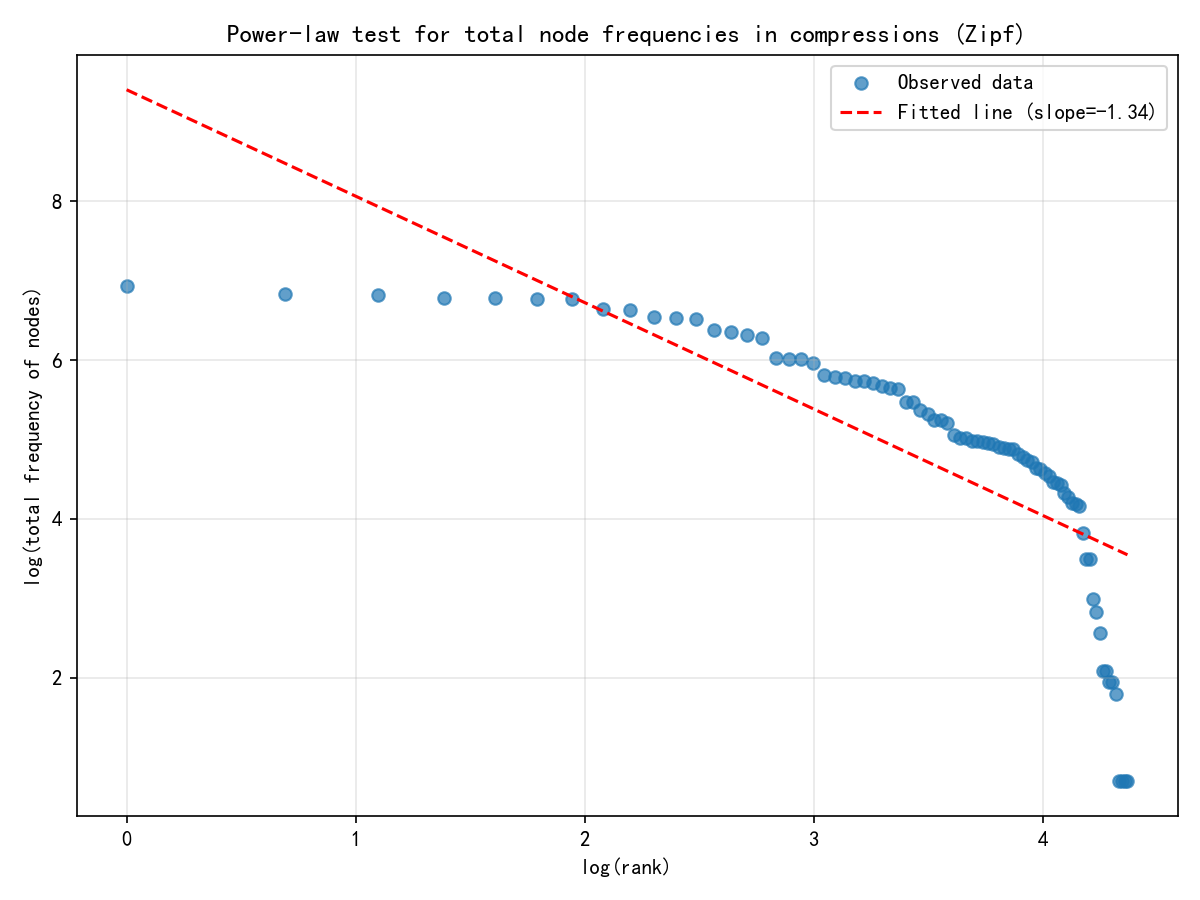
\includegraphics[width=\textwidth]{zipf_node_total.png}
    \caption{节点总出现次数}
    \label{fig:zipf_total}
\end{subfigure}
\caption{概念在压缩事件中出现频率的双对数分布及其幂律拟合。横轴：按频率降序排列的排名 $r$（对数坐标），纵轴：频率 $f(r)$（对数坐标）。散点为实际观测值，直线为最小二乘线性拟合（即幂律 $f(r)\propto r^{-\alpha}$）。（a）中心节点出现次数：统计了 3376 次压缩事件中 32 个不同中心节点的出现频率，幂律指数 $\alpha=-1.360$，拟合优度 $R^2=0.654$，$p=2.1\times10^{-8}$。（b）节点总出现次数：统计了 21469 次出现中 79 个节点的频率，幂律指数 $\alpha=-1.341$，$R^2=0.602$，$p=4.6\times10^{-17}$。两个分布均表明少数核心概念（如“算法”“操作系统”）主导了压缩过程，体现了能量最小化驱动下认知网络自发形成的无标度结构，与自然语言词频的 Zipf 定律高度相似。}
\label{fig:zipf_distributions}
\end{figure}

两个分布均表现出与幂律一致的显著特征，关键统计量汇总于表 \ref{tab:zipf_stats}。

\begin{table}[H]
\centering
\caption{概念出现频率的幂律拟合结果}
\label{tab:zipf_stats}
\begin{tabular}{lcccc}
\toprule
\textbf{指标} & \textbf{幂律指数（斜率）} & \textbf{拟合优度 $R^2$} & \textbf{$p$ 值} & \textbf{事件总数} \\
\midrule
中心节点出现次数 & $-1.360$ & 0.654 & $2.1\times10^{-8}$ & 3376 \\
节点总出现次数   & $-1.341$ & 0.602 & $4.6\times10^{-17}$ & 21469 \\
\bottomrule
\end{tabular}
\end{table}

中心节点出现次数（共3376次压缩事件，涉及32个不同中心）的分布揭示了系统中的一个重要现象：少数概念（如“算法”“操作系统”“相对论”）被反复选为压缩中心，而大多数概念极少成为中心。节点总出现次数（21469次出现，涉及79个节点）的分布则刻画了概念在压缩活动中整体活跃度的不均衡性——通用性强的抽象概念频繁参与压缩，而具体领域概念则较少被卷入。这种分布模式是复杂系统中典型的“富者愈富”现象的外在表现。

这两个分布特征与复杂系统中的无标度网络高度一致 \citep{newman2005power}，且其统计规律（幂指数接近 $-1$）与经典 Zipf 定律 \citep{zipf1949human} 存在有趣的对应。在认知领域，学习曲线也常呈现幂律形式 \citep{anderson2001power}，这为本模型与人类认知规律的关联提供了一个新的观察视角。重要的是，这些统计规律并非由外部预设规则产生，而是能量最小化驱动下系统自发演化的结果。它们从结构组织层面为模型的认知合理性提供了新的观察证据：认知系统在追求能量最优的过程中，自然演化出了枢纽节点主导、多数节点稀疏参与的核心-边缘结构，这与人类认知中“核心概念”的固化过程以及语言使用的统计规律存在深刻的对应关系。

此外，这一分布特征也佐证了第 6.5 节中观察到的相变行为——当系统跨越临界点后，少数原理性节点开始主导压缩与迁移，使得宏观结构呈现出无标度特征。这一发现将能量动力学与复杂系统理论联系起来，暗示能量最小化可能是认知复杂系统自组织临界性的一种深层驱动力。

% ========== SECTION 8: 讨论 ==========
\section{讨论}

% ========== SUBSECTION 8.1: 理论意义与观察 ==========
\subsection{理论意义与观察}

本研究通过四个规模的思想实验，在不同知识复杂度环境中观察了认知系统的行为模式，从多个维度为认知科学和人工智能理论提供了新的思考角度。

\textbf{规模适应性规律的观察}：从51概念到111概念，自然涌现模型的能耗优化从86.9\%降至47.9\%（降幅45.6\%），而预设算法模型从22.8\%降至7.6\%（降幅67.1\%）。这表明知识复杂度的增加对任何认知系统都构成挑战，但基于能量最小化的自组织机制能更好地应对这种挑战。系统在111概念环境中从丰富的探索性压缩（51概念：466次）转向精准的原理性整合（111概念：43次），压缩密度从9.14次/概念降至0.39次/概念，反映了从广泛试探到精准整合的策略转变。

\textbf{能量优化作为组织原则的普适性}：在不同概念规模下，能量最小化始终表现为认知组织的有效驱动力。自然涌现模型在四个规模中分别实现86.9\%、72.3\%、61.4\%和47.9\%的能耗优化，显著优于预设算法模型。更重要的是，涌现模型的规模衰减幅度（45.6\%）远小于预设算法模型（67.1\%）和Q-learning模型（78.5\%），提示基于能量最小化的自然演化机制在处理认知复杂度增长时具有更好的适应性。

\textbf{创造性思维模式的涌现特征}：实验观察到创造性思维的某些特征以不同方式呈现：低复杂度环境下广泛建立概念连接但迁移尚未形成（积累阶段）；中等复杂度环境下开始出现跨领域迁移（探索阶段）；高复杂度环境下迁移极其谨慎、压缩高度精准（巩固阶段）。这些模式与Wallas的创造性思维四阶段理论存在有趣的呼应，且驱动力始终是能量最小化。

\textbf{幂律分布揭示的认知无标度特征。}除了宏观能耗演化，系统的微观结构同样呈现出深刻的统计规律。我们对所有自然涌现压缩事件中概念的出现频率进行了分析，发现中心节点出现次数和节点总出现次数均表现出与幂律一致的分布特征（图 \ref{fig:zipf_distributions}，表 \ref{tab:zipf_stats}）。这种“少数枢纽节点频繁使用、多数节点稀疏参与”的分布模式，是复杂系统自组织临界性和无标度网络结构的典型特征。在自然语言中，单词使用频率同样服从Zipf分布 \citep{zipf1949human}，而本模型中的概念频率分布与之高度相似，这为能量最小化驱动下的认知演化自发产生了与人类语言使用相通的统计规律提供了一个有趣的观察窗口。 这一发现为模型的认知合理性提供了独立于能耗指标的观察证据：系统不仅在能量层面实现了优化，其结构组织方式也与真实认知系统（如语义网络）具有统计上的一致性。幂律分布的存在也佐证了第6.5节中观察到的相变行为——当系统跨越临界点后，少数原理性节点开始主导压缩与迁移，使得宏观结构呈现出无标度特征。能量最小化原则由此将认知动力学与复杂系统理论联系起来，提示它可能是认知复杂系统自组织临界性的一种深层驱动力。

% ========== SUBSECTION 8.2: 对下一代人工智能的范式启示 ==========
\subsection{对下一代人工智能的范式启示}

Bowers等人对当前AI与人类认知对比研究的方法论问题提出了批评。本文的观察为这一批评提供了一个可能的出路：从数据驱动转向原理驱动，从统计关联转向结构理解。

\textbf{从预设架构到自然演化。}预设算法模型在111概念环境中性能显著下降至7.6%，而自然涌现模型仍保持47.9%的强劲表现，提示基于自然演化的架构比预设算法更具扩展性。这一观察挑战了当前AI系统依赖预设架构和规则的设计哲学，暗示应更多考虑向自组织、自适应的系统设计方向探索。

\textbf{从统计关联到原理理解。}实验中的高质量迁移均基于抽象原理（如“模式识别”）而非表面相似性，且相同迁移路径在不同规模下重复出现。这提示下一代AI或可注重原理性理解而非仅统计关联，通过识别深层结构相似性实现更有效的跨领域迁移。

\textbf{与当前AI前沿的对话：从数据驱动到原理驱动。}近期学术界对人工智能发展的反思指出：大模型已逼近人类数据边界，真正的智能应像婴儿在感知行动中自我学习。本文的自然涌现模型完全不依赖于大规模训练数据，仅从“认知时空”和“能量动力学”两个基本公设出发，通过能量最小化原理自发产生概念压缩和原理迁移，实现了一种生成性学习而非数据拟合的雏形。实验结果展示了这一方向的潜力：在111概念的复杂认知环境中，自然涌现模型仍实现47.9%的能耗降低，而传统预设算法仅7.6%。更重要的是，这种优化是自发的、无监督的，不需要针对特定任务的标注数据。实验中的概念压缩（如“操作系统+数据结构+网络+软件工程”的深度整合）和原理迁移（如“模式识别”在不同领域的桥梁作用）体现了系统的洞察力——不是表面的关联，而是深层的原理性理解。这种基于原理的认知框架天然支持无限任务，因为它建立的是通用的认知能力而非特定的任务技能。

\textbf{认知负荷的自适应管理。}系统在111概念环境中自发将压缩密度从9.14降至0.39次/概念，迁移从多次降至仅1次，展现了认知负荷的智能管理能力。这对设计可扩展的AI系统具有启示：系统若能根据任务复杂度自动调整其认知策略，可能有助于避免在复杂环境中陷入计算困境。

\textbf{代数结构的显式建模。}认知操作的群论描述为AI提供了新的数学基础。基于代数结构的认知模型可能为当前神经网络的可解释性困境提供新思路，通过数学结构提供对认知过程的严格描述。

% ========== SUBSECTION 8.3: 与神经科学的联系 ==========
\subsection{与神经科学的联系}

我们的理论框架与神经科学的多个前沿发现形成了有趣的对应关系。能量效率原则与人脑仅占体重2\%却消耗20\%基础代谢率的能量预算相呼应；概念压缩密度随规模衰减的现象与发育过程中突触修剪的过程存在类比；模块化组织的结构对应大脑功能模块的自然边界；神经可塑性的动力学模拟则与长时程增强、长时程抑制等机制形成映射。这些对应关系提示，能量最小化可能不仅是认知层面的组织原则，也可能是神经层面结构优化的普遍原理。Carlson等人 \cite{carlson2025attending} 的综述展示了认知科学在现实问题（如气候变化关注）中的应用，进一步凸显了认知研究的跨学科价值。

% ========== SUBSECTION 8.4: 局限性与未来工作 ==========
\subsection{局限性与未来工作}

尽管本研究在认知计算建模方面取得了一些观察结果，但仍存在若干局限性，这些局限性同时也指明了未来研究的方向。

\textbf{网络规模与真实认知的差距}：即使111概念网络，与人类专家的知识体系相比仍然规模有限；概念节点采用简洁定义，缺乏真实知识中的层次结构和模糊性；元结构映射带有还原论倾向，未能充分体现整体论思维中的横向关联和隐喻张力。未来可整合WordNet、ConceptNet等知识库构建数千概念的认知网络，引入层次化表征和模糊语义，并探索基于汉字偏旁部首的元结构以贴近中文整体论思维。

\textbf{个体差异建模的精细度不足}：当前仅通过随机初始化引入个体差异，缺乏基于认知风格的系统性建模。未来可基于心理学量表建立认知风格参数化模型，模拟从儿童到专家的认知发展连续体。A. Jacobs \cite{jacobs2026cognitive} 提出的“认知压缩风格”概念框架可为个体差异建模提供理论支撑。

\textbf{多模态感知运动的整合缺失}：当前模型完全基于抽象概念，缺乏感知和运动的具身基础。未来可结合多模态神经网络，在机器人平台上实现具身验证。

\textbf{实证验证的广度与深度不足}：当前验证主要基于计算指标，缺乏与人类行为数据和脑成像数据的直接对比。未来需设计心理学实验检验模型预测，并将模型输出与脑活动数据进行多变量模式分析。认知科学的应用前景广阔，如Carlson等 \cite{carlson2025attending} 对气候变化关注的研究所示，认知理论可指导现实问题的解决。

\textbf{理论框架的数学深化需求}：群论应用仍处于概念层面，拓扑性质和动力系统理论未充分挖掘。未来可深化李群李代数描述，应用拓扑数据分析认知空间的拓扑特征，用分岔理论解释认知相变现象。

\textbf{语境动态性与跨文化扩展}：当前模型基于单一静态语境假设，未来可引入语境演化算子，构建“语境-知识”联合演化系统。通过中英文双语认知网络的对比，检验认知图论的跨文化普适性，为文化心理学提供计算模型支撑。

\textbf{概念频率分布的进一步探索与验证。}尽管我们观察到概念出现频率与幂律分布存在一致性，但当前分析仍存在若干局限：首先，概念集合规模有限（111 概念中仅 79 个节点参与压缩事件），可能影响分布的稳定性，未来可在数千概念的大规模网络中重复检验这一现象；其次，幂律指数（$-1.36$ 左右）与经典语言 Zipf 指数（$-1$ \citep{zipf1949human}）的差异，可能源于语义相似度计算方式、压缩阈值设定或概念定义粒度的影响，需要通过参数敏感性分析和跨领域对比进一步探究其成因；最后，本研究仅验证了与幂律分布的一致性，尚未与其他分布（如指数分布、对数正态分布）进行严格比较，未来应引入更系统的统计方法（如 Clauset 等 \citep{clauset2009power} 提出的框架）来探讨幂律是否为这些分布的最佳描述模型。此外，概念频率的跨文化对比（如中英文认知网络）也将有助于检验这一分布规律的普适性。

% ========== SECTION 9: 结论 ==========
\section{结论}

本文通过一组思想实验，在不同知识复杂度的环境中观察了认知图论框架下能量优化驱动的认知组织现象。基于51、71、91和111个跨领域概念的四个规模实验，我们观察到以下核心现象：

\begin{enumerate}
\item \textbf{能量最小化作为认知组织的基本原则}：自然涌现模型在四个规模中分别实现86.9\%、72.3\%、61.4\%和47.9\%的能耗优化，而预设算法模型仅为22.8\%、15.5\%、12.2\%和7.6\%。两者之间的显著差异提示能量最小化是一种更根本的认知组织原则，其有效性随知识复杂度增长仍保持稳健。

\item \textbf{概念压缩密度随规模自适应衰减}：系统自发形成的概念压缩密度从51概念的9.14次/概念骤降至111概念的0.39次/概念（降幅95.7\%）。这一趋势与人类从广泛探索到精准整合的认知发展过程存在有趣的对应，反映了系统在面对不同知识密度时的自适应策略调整——低密度环境中广泛试探，高密度环境中形成深度整合。

\item \textbf{原理迁移的涌现窗口与稳定性}：迁移次数在中等复杂度时达到峰值（71/91概念各3次），111概念时仅剩1次，而迁移效率稳定在0.35-0.45之间。“模式识别”作为核心原理节点，在7次迁移中出现6次，彰显了抽象原理在跨领域连接中的关键作用。相同迁移路径在不同规模下的重复出现（如发展心理学→模式识别→元认知）提示其有效性经过环境筛选。

\item \textbf{111概念临界现象}：在111概念环境中，系统策略发生根本性转变——概念压缩从301次骤降至43次，原理迁移仅发生1次。这暗示认知系统在极端复杂度下会触发策略相变，从“探索性整合”转向“保守性维持”，只保留最必要的整合与迁移。

\item \textbf{压缩势的稳定性证实了能量最小化的统一驱动力}：尽管概念压缩次数随规模下降，但被压缩集群的压缩势始终稳定在 0.8 左右，且标准差随规模减小，表明系统在不同复杂度下对“好压缩”的内在标准一致，并从广泛探索转向精准整合。

\item \textbf{概念出现频率的幂律分布揭示了认知系统的无标度特征。}中心节点和节点总出现次数的分布均与幂律高度一致（$R^2>0.6$，$p<10^{-8}$），表明能量最小化驱动下的认知网络自发演化出了少数枢纽节点主导、多数节点稀疏参与的核心-边缘结构。这一统计规律与自然语言中的 Zipf 定律 \citep{zipf1949human} 高度相似，为模型的认知合理性提供了独立于能耗指标的跨领域观察证据。

\end{enumerate}

这些观察为理解人类认知的组织方式提供了新的理论视角：认知系统通过能量最小化这一第一性原理，自发形成概念压缩与原理迁移等高阶功能，并能够根据知识复杂度自适应调整认知策略。本工作也揭示了从“数据驱动”到“原理驱动”的AI范式转变的可能性——为机器赋予内在的“认知能耗”感知与优化能力，让AI从统计关联走向结构理解，从机械执行走向创造性思维。基于能量优化的认知图论框架，为实现这一愿景提供了初步的理论基础与探索路径。

\newpage

% ========== REFERENCES ==========
\bibliography{references}
% \begin{thebibliography}{99}
% \bibitem{anderson2004act} Anderson, J. R. (2004). How can the human mind occur in the physical universe? Oxford University Press.
% \bibitem{vaswani2017attention} Vaswani, A., et al. (2017). Attention is all you need. In \textit{Advances in Neural Information Processing Systems}.
% \bibitem{lecun2015deep} LeCun, Y., Bengio, Y., \& Hinton, G. (2015). Deep learning. \textit{Nature}, 521(7553), 436-444.
% \bibitem{sutton2018reinforcement} Sutton, R. S., \& Barto, A. G. (2018). Reinforcement learning: An introduction. MIT press.
% \bibitem{friston2010free} Friston, K. (2010). The free-energy principle: a unified brain theory? \textit{Nature Reviews Neuroscience}, 11(2), 127-138.
% \bibitem{tenenbaum2011grow} Tenenbaum, J. B., et al. (2011). How to grow a mind: Statistics, structure, and abstraction. \textit{Science}, 331(6022), 1279-1285.
% \bibitem{gardenfors2004conceptual} Gärdenfors, P. (2004). Conceptual spaces: The geometry of thought. MIT press.
% \bibitem{rotman1995theory} Rotman, J. J. (1995). An introduction to the theory of groups. Springer Science \& Business Media.
% \bibitem{newell1972human} Newell, A., \& Simon, H. A. (1972). Human problem solving. Prentice-Hall.
% \bibitem{song2018survey} Song, P., Wang, X., \& Li, H. (2018). A survey of knowledge graph construction and application. \textit{IEEE Access}, 6, 77529-77540.
% \bibitem{shepard1987universals} Shepard, R. N. (1987). Toward a universal law of generalization for psychological science. \textit{Science}, 237(4820), 1317-1323.
%\bibitem{glazebrook2009small} Glazebrook, J. F., \& Wallace, R. (2009). Small worlds and Red Queens in the Global Workspace: An information-theoretic approach. \textit{Cognitive Systems Research}, 10(4), 333-365.
% \bibitem{bowers2023importance} Bowers, J. S., et al. (2023). On the importance of severely testing deep learning models of cognition. \textit{Cognitive Systems Research}, 82, 101158.
% \bibitem{woensdregt2024lessons} Woensdregt, M., et al. (2024). Lessons for Theory from Scientific Domains Where Evidence is Sparse or Indirect. \textit{Computational Brain \& Behavior}, 7(4), 521-538.
% \end{thebibliography}

\newpage

% ========== APPENDIX ==========
\appendix

% ========== APPENDIX A: 代数框架验证细节 ==========
\section{代数框架验证细节}
\label{app:algebraic_validation}

本附录提供第5节所述代数框架验证实验的详细设置、数据和结果。

% ========== A.1 实验设计 ==========
\subsection{实验设计}

\textbf{实验1：认知操作半群验证}
\begin{itemize}
    \item 目的：观察基本认知操作（遍历、学习、遗忘、压缩、迁移）在复合下是否满足半群性质。
    \item 方法：随机生成13种认知操作，测试结合律$(a \circ b) \circ c = a \circ (b \circ c)$。
\end{itemize}

\textbf{实验2：Noether型对应观察}
\begin{itemize}
    \item 目的：观察认知对称性与守恒量之间的对应关系。
    \item 方法：在5节点、10节点、15节点三个认知网络上检测对称性并计算守恒量（全局能量、结构熵、分形维数）的相对变化。
\end{itemize}

\textbf{实验3：轨道-稳定子定理适用性观察}
\begin{itemize}
    \item 目的：观察轨道-稳定子定理在认知状态空间中的表现。
    \item 方法：计算认知对称群大小$|\cognitivegroup|$、稳定子大小$|Stab(G)|$和轨道大小$|O_G|$，验证$|O_G| = \frac{|\cognitivegroup|}{|Stab(G)|}$。
\end{itemize}

\textbf{实验4：李群演化框架演示}
\begin{itemize}
    \item 目的：展示连续时间认知演化的李群描述的可行性。
    \item 方法：采用三种不同的李代数生成元组合（能量优化主导、概念压缩主导、原理迁移主导），观测演化前后的认知能耗变化。
\end{itemize}

\textbf{实验5：代数方法可扩展性测试}
\begin{itemize}
    \item 目的：评估代数方法在不同规模网络中的计算效率。
    \item 方法：在5、8、10、12、15节点网络上测试半群运算和对称性检测时间。
\end{itemize}

% ========== A.2 实验结果 ==========
\subsection{实验结果}

\textbf{认知操作半群验证}：所有13种操作的组合测试均满足结合律，关键案例如下：
\begin{itemize}
    \item (学习 $\circ$ 遗忘) $\circ$ 遍历 = 学习 $\circ$ (遗忘 $\circ$ 遍历)
    \item (压缩 $\circ$ 迁移) $\circ$ 学习 = 压缩 $\circ$ (迁移 $\circ$ 学习)
    \item (遍历 $\circ$ 学习) $\circ$ 遗忘 = 遍历 $\circ$ (学习 $\circ$ 遗忘)
\end{itemize}

\textbf{Noether型对应观察}：结果见表\ref{tab:app_noether}。三个网络均表现出能量守恒趋势（相对变化<1\%），结构熵完全守恒，分形维数微小变化。网络同构数均为1（仅恒等映射），体现了认知系统的个体独特性。

\begin{table}[H]
\centering
\caption{Noether型对应观察结果}
\label{tab:app_noether}
\begin{tabular}{lcccc}
\toprule
\textbf{网络} & \textbf{同构数} & \textbf{能量守恒趋势} & \textbf{结构熵守恒} & \textbf{分形维数趋势保持} \\
\midrule
网络1 (5节点) & 1 & 是 & 是 & 是 \\
网络2 (10节点) & 1 & 是 & 是 & 是 \\
网络3 (15节点) & 1 & 是 & 是 & 是 \\
\bottomrule
\end{tabular}
\end{table}

\textbf{轨道-稳定子定理适用性}：由于网络同构群大小均为1，稳定子大小和轨道大小均为1，定理平凡成立（$1 = 1/1$）。

\textbf{李群演化框架}：三种策略的能耗变化见表\ref{tab:app_lie}。能量优化主导策略实现了最大能耗降低（34.7\%）。

\begin{table}[H]
\centering
\caption{李群演化策略的能耗变化}
\label{tab:app_lie}
\begin{tabular}{lcc}
\toprule
\textbf{策略类型} & \textbf{生成元系数} & \textbf{能耗变化} \\
\midrule
能量优化主导 & $\{\mathcal{E}:0.7, \mathcal{C}:0.2, \mathcal{M}:0.1\}$ & -34.7\% \\
概念压缩主导 & $\{\mathcal{E}:0.3, \mathcal{C}:0.6, \mathcal{M}:0.1\}$ & -14.7\% \\
原理迁移主导 & $\{\mathcal{E}:0.2, \mathcal{C}:0.2, \mathcal{M}:0.6\}$ & -12.4\% \\
\bottomrule
\end{tabular}
\end{table}

\textbf{可扩展性测试}：结果见表\ref{tab:app_scalability}。在15节点内所有运算时间小于0.1秒，对称性检测复杂度为$O(n!)$，但通过启发式算法可优化。

\begin{table}[H]
\centering
\caption{代数方法可扩展性测试结果}
\label{tab:app_scalability}
\begin{tabular}{lccc}
\toprule
\textbf{网络规模} & \textbf{半群运算时间(s)} & \textbf{对称性检测时间(s)} & \textbf{同构数} \\
\midrule
5节点 & 0.0000 & 0.0060 & 1 \\
8节点 & 0.0000 & 0.0620 & 1 \\
10节点 & 0.0000 & 0.0260 & 1 \\
12节点 & 0.0000 & 0.0450 & 1 \\
15节点 & 0.0000 & 0.0072 & 1 \\
\bottomrule
\end{tabular}
\end{table}

% ========== APPENDIX B: 预设算法模型实现 ==========
\section{预设算法模型实现}
\label{app:preset_model}

本附录提供第 2.1 节中作为对照基线的预设算法模型的核心实现。该模型基于 Python 实现，包含显式的认知状态管理和基于规则的操作选择机制。以下代码片段摘取自项目源文件 \texttt{cognitive\_graph.py}、\texttt{cognitive\_states.py} 和 \texttt{enhanced\_model.py}，并附有参数说明。所有硬编码数值均直接取自源代码，确保与实验运行版本一致。

\subsection{认知状态管理}
认知状态由 \texttt{CognitiveState} 枚举和 \texttt{CognitiveStateManager} 类管理。状态转移矩阵定义于外部配置文件 \texttt{config.py}（实验中采用马尔可夫链设计，具体概率见表 B.1）。主观能耗在状态变化时根据状态对应的能耗范围随机更新。

\begin{lstlisting}[language=Python, caption={认知状态枚举与管理器（\texttt{cognitive\_states.py}）}, label=lst:state_manager]
from enum import Enum
import random
from config import STATE_TRANSITION_MATRIX, STATE_ENERGY_RANGES

class CognitiveState(Enum):
    FOCUSED = "专注状态"
    EXPLORATORY = "探索状态"
    FATIGUED = "疲劳状态"
    INSPIRED = "灵感状态"

class CognitiveStateManager:
    def __init__(self):
        self.current_state = CognitiveState.FOCUSED
        self.subjective_energy = 1.5                     # 初始主观能耗
        self.cognitive_energy_history = []

    def update_cognitive_state(self):
        current_state_name = self.current_state.name
        transition_probs = STATE_TRANSITION_MATRIX[current_state_name]
        rand_val = random.random()
        cumulative_prob = 0
        for new_state_name, prob in transition_probs.items():
            cumulative_prob += prob
            if rand_val <= cumulative_prob:
                new_state = CognitiveState[new_state_name]
                if new_state != self.current_state:
                    self.current_state = new_state
                    self._update_subjective_energy()
                break
        # 记录历史（略）

    def _update_subjective_energy(self):
        state_name = self.current_state.name
        energy_range = STATE_ENERGY_RANGES[state_name]
        self.subjective_energy = random.uniform(energy_range[0], energy_range[1])
        self.subjective_energy = max(0.1, min(3.0, self.subjective_energy))
\end{lstlisting}

实验中使用的状态转移矩阵和能耗范围如表 B.1 和表 B.2 所示（数值取自实验配置文件，与论文第 7.1 节参数一致）。

\begin{table}[H]
\centering
\caption{状态转移概率矩阵（取自 \texttt{config.py}）}
\label{tab:state_transition_app}
\begin{tabular}{lcccc}
\toprule
\textbf{当前状态} & \textbf{FOCUSED} & \textbf{EXPLORATORY} & \textbf{INSPIRED} & \textbf{FATIGUED} \\
\midrule
FOCUSED      & 0.6 & 0.2 & 0.1 & 0.1 \\
EXPLORATORY  & 0.3 & 0.5 & 0.1 & 0.1 \\
INSPIRED     & 0.4 & 0.3 & 0.2 & 0.1 \\
FATIGUED     & 0.3 & 0.2 & 0.1 & 0.4 \\
\bottomrule
\end{tabular}
\end{table}

\begin{table}[H]
\centering
\caption{各状态主观能耗范围（取自 \texttt{config.py}）}
\label{tab:energy_ranges_app}
\begin{tabular}{lc}
\toprule
\textbf{状态} & \textbf{能耗范围} \\
\midrule
FOCUSED      & [1.2, 1.8] \\
EXPLORATORY  & [1.5, 2.2] \\
INSPIRED     & [0.8, 1.5] \\
FATIGUED     & [0.5, 1.0] \\
\bottomrule
\end{tabular}
\end{table}

\subsection{基础认知图核心操作}
\texttt{BaseCognitiveGraph} 类实现了遍历、遗忘、压缩、迁移等核心操作。以下展示操作选择机制和遍历方法的关键代码。

\begin{lstlisting}[language=Python, caption={操作选择与遍历（\texttt{cognitive\_graph.py}）}, label=lst:operations]
class BaseCognitiveGraph:
    def _select_operation_based_on_state(self):
        """根据当前状态选择操作，概率硬编码于方法内。"""
        state_operations = {
            CognitiveState.FOCUSED: {
                "hard_traversal": 0.5, "soft_traversal": 0.3,
                "compression": 0.1, "migration": 0.1
            },
            CognitiveState.EXPLORATORY: {
                "hard_traversal": 0.3, "soft_traversal": 0.4,
                "compression": 0.1, "migration": 0.2
            },
            CognitiveState.FATIGUED: {
                "hard_traversal": 0.2, "soft_traversal": 0.4,
                "compression": 0.2, "migration": 0.2
            },
            CognitiveState.INSPIRED: {
                "hard_traversal": 0.3, "soft_traversal": 0.4,
                "compression": 0.1, "migration": 0.2
            }
        }
        probs = state_operations[self.current_state]
        # 随机选择（略）
    
    def traverse_path(self, path, traversal_type="hard"):
        """沿路径遍历，更新边权重（学习效应）。"""
        # 能量检查、学习率计算等
        for i in range(len(path)-1):
            u, v = path[i], path[i+1]
            # 更新遍历计数
            self.G[u][v]['traversal_count'] += 1
            similarity = 0.5  # 实际应由语义网络提供
            base_rate = self.base_learning_rate  # 默认0.85
            if traversal_type == "hard":
                learning_rate = base_rate * (0.7 + 0.3 * similarity)
            else:
                learning_rate = base_rate * 0.9
            # 应用个体变异
            learning_rate *= np.random.uniform(1 - self.learning_rate_variation,
                                                1 + self.learning_rate_variation)
            current_weight = self.G[u][v]['weight']
            new_weight = max(0.05, current_weight * (1 - learning_rate * (current_weight/2.0)))
            self.G[u][v]['weight'] = new_weight
        # 更新认知状态（略）
    
    def forgetting_function(self, current_time, last_activation_time, current_energy, similarity):
        """指数遗忘模型。"""
        time_gap = current_time - last_activation_time
        base_forgetting = 1 - math.exp(-time_gap / 500)
        energy_factor = 0.5 + 0.5 * (current_energy / 2.0)
        similarity_protection = 1 - (similarity * 0.5)
        forgetting_factor = base_forgetting * energy_factor * similarity_protection * self.forgetting_rate
        return min(forgetting_factor, 0.1)
\end{lstlisting}

\subsection{语义增强与能耗优化扩展}
\texttt{enhanced\_model.py} 中的子类提供了基于语义相似度的初始化和智能压缩功能。

\begin{lstlisting}[language=Python, caption={语义增强与能耗优化类（\texttt{enhanced\_model.py}）}, label=lst:enhanced]
class SemanticEnhancedCognitiveGraph(BaseCognitiveGraph):
    def initialize_semantic_graph(self):
        """基于语义相似度初始化边权重。"""
        nodes = list(self.semantic_network.concept_definitions.keys())
        self.G.add_nodes_from(nodes)
        for i, node1 in enumerate(nodes):
            for node2 in nodes[i+1:]:
                similarity = self.calculate_semantic_similarity(node1, node2)
                if similarity > 0.1:  # 相似度阈值
                    energy = 2.0 - similarity * 1.5
                    energy = max(0.3, min(2.0, energy))
                    self.G.add_edge(node1, node2, weight=energy, 
                                    original_weight=energy, traversal_count=0)
    
    def conceptual_compression_based_on_semantics(self, compression_threshold=0.3):
        """根据语义相似度寻找可压缩集群。"""
        # 寻找相似节点组，调用父类的 conceptual_compression 方法
        # 阈值 0.3 取自参数默认值

class EnergyOptimizedCognitiveGraph(SemanticEnhancedCognitiveGraph):
    def smart_concept_compression(self, compression_threshold=0.4):
        """智能压缩：仅当预期能耗节省超过阈值时才执行。"""
        high_energy_clusters = self._find_high_energy_clusters()
        for center, nodes in high_energy_clusters:
            if len(nodes) >= 2:
                expected_saving = self._calculate_compression_saving(center, nodes)
                if expected_saving > self.energy_optimization_threshold:  # 默认 0.3
                    self.conceptual_compression(center, nodes, 0.5)
    
    def _calculate_compression_saving(self, center, nodes):
        """计算压缩预期节省比例（假设压缩后能耗降低40%）。"""
        current_total = sum(self.G[center][n]['weight'] for n in nodes if self.G.has_edge(center, n))
        compressed_total = current_total * 0.6  # 经验假设
        return (current_total - compressed_total) / current_total if current_total > 0 else 0
\end{lstlisting}

\subsection{模型参数总结}
预设算法模型中使用的关键参数均直接取自上述代码，汇总于表 B.3。

\begin{table}[H]
\centering
\caption{预设算法模型核心参数}
\label{tab:preset_params}
\begin{tabular}{lll}
\toprule
\textbf{参数名} & \textbf{值} & \textbf{来源} \\
\midrule
初始主观能耗 & 1.5 & \texttt{CognitiveStateManager.\_\_init\_\_} \\
遗忘率 & 0.002 & \texttt{individual\_params} 默认值 \\
基础学习率 & 0.85 & \texttt{individual\_params} 默认值 \\
学习率变异系数 & 0.1 & \texttt{individual\_params} 默认值 \\
语义相似度阈值 & 0.1 & \texttt{initialize\_semantic\_graph} 中的判断条件 \\
压缩阈值（语义） & 0.3 & \texttt{conceptual\_compression\_based}  \\
 &  & \texttt{\_on\_semantics} 参数默认值 \\
压缩阈值（能耗） & 0.4 & \texttt{smart\_concept\_compression} 参数默认值 \\
压缩后能耗假设 & 原能耗的60\% & \texttt{\_calculate\_compression\_saving}  \\
 &  & 中的经验假设 \\
\bottomrule
\end{tabular}
\end{table}

\subsection{主循环逻辑}
模型的每次迭代执行以下步骤（源自 \texttt{BaseCognitiveGraph.monte}）

\noindent
 \texttt{\_carlo\_iteration}:

\begin{enumerate}
    \item 每 100 步更新一次认知状态（\texttt{update\_cognitive\_state}）。
    \item 应用遗忘机制（\texttt{\_apply\_forgetting}）。
    \item 记录当前网络平均能耗。
    \item 根据当前状态选择操作（\texttt{\_select\_operation\_based\_on\_state}）并执行相应函数（硬遍历、软遍历、压缩、迁移）。
\end{enumerate}
迭代共进行 10,000 次，与第 7.1 节实验设置一致。

以上代码和参数完整反映了预设算法模型的设计。实验运行结果（如能耗降低率）已在第 7.2 节中与自然涌现模型对比。

% ========== APPENDIX C: 补充实验数据 ==========
\section{补充实验数据}
\label{app:supplementary_data}

本附录提供第7章中未详细列出的补充数据，包括多层次对比结果、认知状态分布、以及所有压缩与迁移案例。

% ========== C.1 多层次对比实验结果 ==========
\subsection{多层次对比实验结果}

表\ref{tab:app_multi_comparison}展示了随机网络、Q-learning、预设算法模型和自然涌现模型在四个规模下的能耗改善率完整数据。

\begin{table}[H]
\centering
\caption{多层次对比实验结果}
\label{tab:app_multi_comparison}
\begin{tabular}{lcccc}
\toprule
\textbf{模型类型} & \textbf{51概念} & \textbf{71概念} & \textbf{91概念} & \textbf{111概念} \\
\midrule
随机网络 & -61.7\% & -31.6\% & -18.2\% & -12.9\% \\
简单Q-learning & 14.5\% & 7.3\% & 4.0\% & 2.9\% \\
预设算法模型 & 22.8\% & 15.5\% & 12.2\% & 7.6\% \\
自然涌现模型 & 86.9\% & 72.3\% & 61.4\% & 47.9\% \\
\bottomrule
\end{tabular}
\end{table}

% ========== C.2 认知状态分布 ==========
\subsection{预设算法模型的认知状态分布}

表\ref{tab:app_state_dist}为预设算法模型在不同规模下的认知状态分布。

\begin{table}[H]
\centering
\caption{预设算法模型的认知状态分布}
\label{tab:app_state_dist}
\begin{tabular}{lcccc}
\toprule
\textbf{概念规模} & \textbf{专注状态} & \textbf{探索状态} & \textbf{灵感状态} & \textbf{疲劳状态} \\
\midrule
51概念 & 38.9\% & 28.2\% & 21.9\% & 11.0\% \\
71概念 & 37.2\% & 30.8\% & 22.1\% & 9.9\% \\
91概念 & 36.6\% & 29.6\% & 23.7\% & 10.1\% \\
111概念 & 35.0\% & 31.1\% & 23.0\% & 10.9\% \\
\bottomrule
\end{tabular}
\end{table}

% ========== C.3 所有概念压缩案例 ==========
\subsection{所有概念压缩案例}

由于篇幅限制，此处仅列出各规模下的代表性压缩案例（涌现强度前5）。完整案例列表可联系作者获取。

\begin{table}[H]
\centering
\caption{代表性概念压缩案例}
\label{tab:app_compression_cases}
\begin{tabular}{p{2.5cm}p{1cm}p{4.5cm}p{2cm}}
\toprule
\textbf{中心节点} & \textbf{规模} & \textbf{相关节点（部分）} & \textbf{涌现强度} \\
\midrule
算法 & 51 & 自然语言处理, 数据结构, 操作系统, 分布式系统 & 0.801 \\
万有引力 & 51 & 能量守恒, 运动学, 力学, 量子力学 & 0.807 \\
量子力学 & 51 & 电磁学, 热力学, 万有引力, 静电力 & 0.836 \\
\addlinespace
强化学习 & 71 & 迁移学习, 智能体, 生成对抗网络, 模式识别 & 0.825 \\
元认知 & 71 & 语言习得, 发展心理学, 社会认知, 认知负荷 & 0.789 \\
\addlinespace
认知负荷 & 91 & 心理理论, 具身认知, 工作记忆, 决策理论 & 0.819 \\
逻辑学 & 91 & 语言哲学, 伦理学, 本体论, 科学哲学 & 0.812 \\
\addlinespace
操作系统 & 111 & 数据结构, 计算机网络, 软件工程, 数据库, 算法, 分布式系统 & 0.967 \\
镜像神经元 & 111 & 神经可塑性, 功能磁共振, 海马体, 抽象 & 0.825 \\
\bottomrule
\end{tabular}
\end{table}

% ========== C.4 所有原理迁移案例 ==========
\subsection{所有原理迁移案例}

实验中共观察到7次原理迁移，详见表\ref{tab:app_migration_cases}。

\begin{table}[H]
\centering
\caption{所有原理迁移案例}
\label{tab:app_migration_cases}
\begin{tabular}{p{4cm}p{4.5cm}p{2cm}p{1cm}}
\toprule
\textbf{迁移路径} & \textbf{认知解释} & \textbf{效率增益} & \textbf{规模} \\
\midrule
发展心理学 $\rightarrow$ 模式识别 $\rightarrow$ 元认知 & 发展观察方法迁移到元认知反思 & 0.371 & 71 \\
模式识别 $\rightarrow$ 元认知 $\rightarrow$ 心理理论 & AI感知能力迁移至心理理解 & 0.415 & 71 \\
智能体 $\rightarrow$ 模式识别 $\rightarrow$ 数据挖掘 & 智能体利用模式识别优化数据挖掘 & 0.401 & 71 \\
注意力机制 $\rightarrow$ 专家系统 $\rightarrow$ 模式识别 & 注意力通过专家系统迁移至模式识别 & 0.388 & 71 \\
发展心理学 $\rightarrow$ 模式识别 $\rightarrow$ 元认知 & （重复出现） & 0.356 & 91 \\
模式识别 $\rightarrow$ 元认知 $\rightarrow$ 心理理论 & （重复出现） & 0.393 & 91 \\
生成对抗网络 $\rightarrow$ 模式识别 $\rightarrow$ 机器人学 & 生成模型能力迁移至机器人感知 & 0.381 & 91 \\
生成对抗网络 $\rightarrow$ 神经网络 $\rightarrow$ 迭代 & 生成对抗网络的迭代原理迁移至计算迭代 & 0.352 & 111 \\
\bottomrule
\end{tabular}
\end{table}

% ========== APPENDIX C.5: 概念出现频率的幂律分布检验详细数据 ==========
\subsection{概念出现频率的幂律分布检验详细数据}

本附录提供第 7.10 节中所述幂律分布检验的详细统计数据和原始频数表。两个指标分别反映了概念在压缩事件中的中心性和整体活跃度。

\begin{table}[H]
\centering
\caption{中心节点出现次数的幂律分布统计}
\label{tab:app_zipf_center}
\begin{tabular}{lcc}
\toprule
\textbf{统计量} & \textbf{值} & \textbf{说明} \\
\midrule
幂律指数（斜率） & $-1.360$ & 对数坐标下线性回归的斜率 \\
截距 & $7.457$ & 回归直线在 $y$ 轴上的截距 \\
拟合优度 $R^2$ & $0.654$ & 反映拟合效果 \\
$p$ 值 & $2.13\times10^{-8}$ & 斜率显著性的概率值 \\
总压缩事件数 & $3376$ & 所有压缩事件的总和 \\
不同中心节点数 & $32$ & 成为过压缩中心的不同概念数量 \\
\bottomrule
\end{tabular}
\end{table}

\begin{table}[H]
\centering
\caption{中心节点出现次数排名前10的概念}
\label{tab:app_zipf_center_top10}
\begin{tabular}{lc}
\toprule
\textbf{概念} & \textbf{出现次数} \\
\midrule
算法      & 329 \\
操作系统  & 314 \\
相对论    & 252 \\
能量守恒  & 245 \\
量子力学  & 239 \\
动量      & 217 \\
牛顿定律  & 214 \\
静电力    & 168 \\
万有引力  & 160 \\
摩擦力    & 157 \\
\bottomrule
\end{tabular}
\end{table}

\begin{table}[H]
\centering
\caption{节点在压缩事件中出现总次数的幂律分布统计}
\label{tab:app_zipf_total}
\begin{tabular}{lcc}
\toprule
\textbf{统计量} & \textbf{值} & \textbf{说明} \\
\midrule
幂律指数（斜率） & $-1.341$ & 对数坐标下线性回归的斜率 \\
截距 & $9.408$ & 回归直线在 $y$ 轴上的截距 \\
拟合优度 $R^2$ & $0.602$ & 反映拟合效果 \\
$p$ 值 & $4.63\times10^{-17}$ & 斜率显著性的概率值 \\
总出现次数 & $21469$ & 所有节点在压缩事件中出现的总次数 \\
不同节点数 & $79$ & 参与过压缩事件的不同概念总数 \\
\bottomrule
\end{tabular}
\end{table}

\begin{table}[H]
\centering
\caption{节点总出现次数排名前10的概念}
\label{tab:app_zipf_total_top10}
\begin{tabular}{lc}
\toprule
\textbf{概念} & \textbf{出现次数} \\
\midrule
牛顿定律   & 1028 \\
相对论     & 933  \\
运动学     & 917  \\
动量       & 887  \\
能量守恒   & 886  \\
万有引力   & 874  \\
力学       & 870  \\
静电力     & 768  \\
量子力学   & 764  \\
摩擦力     & 698  \\
\bottomrule
\end{tabular}
\end{table}

以上数据与正文第 7.10 节的图 \ref{fig:zipf_distributions} 和表 \ref{tab:zipf_stats} 互为补充，为概念出现频率的幂律行为提供了完整的统计支持。

\end{document}